\documentclass[11pt]{iopart}
\pdfoutput=1
\usepackage{iopams}
\usepackage{amssymb, epsfig}
%\usepackage{amsmath, amssymb,epsfig}
\usepackage{latexsym}

%\usepackage[hypertex,hyperindex]{hyperref}
\usepackage{showkeys}
\usepackage{graphicx}
\usepackage{color}

\newcommand{\pf}{\mbox{pf}}

\begin{document}

\bibliographystyle{plain}
\def\debproof{\noindent {\bf Proof.} }
\def\finproof{\hfill {\small $\Box$} \\}
%\renewcommand{\theequation}{\arabic{section}.\arabic{equation}}
%\tableofcontents
\makeatletter % `@' now normal "letter"
\@addtoreset{equation}{section}
\makeatother  % `@' is restored as "non-letter"
\renewcommand\theequation{{\thesection}.{\arabic{equation}}}

\title[]{Reverse Time Migration for Extended Obstacles in the Half Space: Elastic Waves}
\author{ Zhiming Chen, Shiqi Zhou }
\address{LSEC, Institute of Computational Mathematics, Academy of
	Mathematics and Systems Science, Chinese Academy of Sciences,
	Beijing 100190, China}

\begin{abstract}
	We consider a reverse time migration method for reconstructing extended
	obstacles in the half space with finite aperture data using elastic waves at a fixed
	frequency. We prove the resolution of the reconstruction method in terms of the
	aperture and the depth of the obstacle embedded in the half space. The resolution
	analysis studied by virtue of point spread function implies that the imaginary part of the cross-correlation imaging function
	always peaks on the boundary of the obstacle. Numerical experiments
	are included to illustrate the powerful imaging quality and to confirm our resolution
	results. 
\end{abstract}
\maketitle
\newcommand{\eps}{\varepsilon}
\newcommand{\RR}{\mathcal{R}}
\newtheorem{lem}{Lemma}[section]
\newtheorem{prop}{Proposition}[section]
\newtheorem{cor}{Corollary}[section]
\newtheorem{thm}{Theorem}[section]
\newtheorem{rem}{Remark}[section]
\newtheorem{alg}{Algorithm}[section]
\newtheorem{assum}{Assumption}[section]
\newtheorem{definition}{Definition}[section]


\newcounter{RomanNumber}
\newcommand{\MyRoman}[1]{\rm\setcounter{RomanNumber}{#1}\Roman{RomanNumber}}

\newcommand{\bL}{\mathbf{L}}
\newcommand{\bH}{\mathbf{H}}
\newcommand{\bW}{\mathbf{W}}
\newcommand{\bP}{\mathbf{P}}
\newcommand{\bQ}{\mathbf{Q}}
\newcommand{\bp}{\mathbf{p}}
\newcommand{\bq}{\mathbf{q}}
\newcommand{\uL}{u_{_{\rm L}}}
\newcommand{\vL}{v_{_{\rm L}}}
\newcommand{\tuL}{\tilde u_{_{\rm L}}}
\newcommand{\tvL}{\tilde v_{_{\rm L}}}
\newcommand{\fL}{f_{_{\rm L}}}
\newcommand{\gL}{g_{_{\rm L}}}
\newcommand{\bpL}{\bp_{_{\rm L}}}
\newcommand{\bqL}{\bq_{_{\rm L}}}
\newcommand{\tbpL}{\tilde{\bp}_{_{\rm L}}}
\newcommand{\tbqL}{\tilde{\bq}_{_{\rm L}}}
\newcommand{\tbpLf}{\tilde{\bp}_{_{\rm L,1}}}
\newcommand{\tbpLs}{\tilde{\bp}_{_{\rm L,2}}}
\newcommand{\tbqLf}{\tilde{\bq}_{_{\rm L,1}}}
\newcommand{\tbqLs}{\tilde{\bq}_{_{\rm L,2}}}
\newcommand{\bn}{\nu}
\newcommand{\bv}{\mathbf{v}}
\newcommand{\om}{\omega}
\newcommand{\pa}{\partial}
\newcommand{\la}{\langle}
\newcommand{\ra}{\rangle}
\newcommand{\lla}{\la{\hskip -2pt}\la}
\newcommand{\rra}{\ra{\hskip -2pt}\ra}
\newcommand{\jj}{\|{\hskip -0.8pt} |}
\newcommand{\al}{\alpha}
\newcommand{\ze}{\zeta}
\newcommand{\si}{\sigma}
\newcommand{\ep}{\varepsilon}
\newcommand{\na}{\nabla}
\newcommand{\vp}{\varphi}
\newcommand{\ga}{\gamma}
\newcommand{\Ga}{\Gamma}
\newcommand{\Om}{\Omega}
\newcommand{\de}{\delta}
\newcommand{\Th}{\Theta}
\newcommand{\De}{\Delta}
\newcommand{\Lam}{\Lambda}
\newcommand{\lam}{\lambda}
\newcommand{\tri}{\triangle}
\newcommand{\lj}{[{\hskip -2pt} [}
\newcommand{\rj}{]{\hskip -2pt} ]}
\newcommand{\bks}{\backslash}
%\newcommand{\diag}{\mathrm{diag}}
\newcommand{\diam}{\mathrm{diam}}
\newcommand{\osc}{\mathrm{osc}}
\newcommand{\meas}{\mathrm{meas}}
\newcommand{\dist}{\mathrm{dist}}

\newcommand{\mL}{\mathscr{L}}
\newcommand{\cT}{{\cal T}}
\newcommand{\cM}{{\cal M}}
\newcommand{\cE}{{\cal E}}
\newcommand{\cL}{{\cal L}}
\newcommand{\cF}{{\cal F}}
\newcommand{\cB}{{\cal B}}
\newcommand{\PML}{{\rm PML}}
\newcommand{\FEM}{{\rm FEM}}
\newcommand{\rd}{\,\mathrm{d}}

\renewcommand{\i}{\mathbf{i}}
\renewcommand{\v}{\mathbf{v}}
\renewcommand{\u}{\mathbf{u}}
\renewcommand{\r}{\mathbf{r}}
\newcommand{\gR}{{\mathbb{R}}}
\newcommand{\Z}{{\mathbb{Z}}}
\newcommand{\C}{{\mathbb{C}}}
\newcommand{\I}{{\mathbb{I}}}
\renewcommand{\Re}{\mathrm{Re}\,}
\renewcommand{\Im}{\mathrm{Im}\,}
\renewcommand{\div}{\mathrm{div}}
\newcommand{\curl}{\mathrm{curl}}
\newcommand{\Curl}{\mathbf{curl}}
\newcommand{\pv}{\mathrm{P.V}}

\newcommand{\Np}{\mathcal{N}_p}
\newcommand{\Ns}{\mathcal{N}_s}
\newcommand{\Tp}{\mathcal{T}_p}
\newcommand{\Ts}{\mathcal{T}_s}
\newcommand{\Na}{\mathcal{N}_\alpha}
\newcommand{\Nb}{\mathcal{N}_\beta}
\newcommand{\Ta}{\mathcal{T}_\alpha}
\newcommand{\Tb}{\mathcal{T}_\beta}
\newcommand{\GG}{\mathcal{G}}

\newcommand{\N}{\mathbb{N}}
\newcommand{\D}{\mathbb{D}}
\newcommand{\T}{\mathbb{T}}
\newcommand{\A}{\mathbb{A}}
\newcommand{\B}{\mathbb{B}}
\newcommand{\G}{\mathbb{G}}
\newcommand{\F}{\mathbb{F}}
\newcommand{\R}{\mathbb{R}}
\newcommand{\W}{\mathbb{W}}
\newcommand{\V}{\mathbb{V}}
\newcommand{\J}{\mathbb{J}}
\newcommand{\Zg}{\mathbb{Z}}
\newcommand{\Gtheta}{\mathbb{\Theta}}
\newcommand{\Gphi}{\mathbb{\Phi}}

%%%%%%%%%%%%%%%%%%%%%%%%%%%%%%%%%%%%%%%%%%%%%%%%%%%%%%%%%%%%%%%%%%%%
\newcommand{\be}{\begin{eqnarray}}
\newcommand{\ee}{\end{eqnarray}}
\newcommand{\ben}{\begin{eqnarray*}}
	\newcommand{\een}{\end{eqnarray*}}
\newcommand{\nn}{\nonumber}

\section{Introduction}\label{section1}
In this paper we study a reverse time migration (RTM) algorithm to find the support of an unknown obstacle in the half space from the measurement of scattered waves on the boundary of the half space which is far away from the obstacle. The physical properties of the obstacle such as penetrable or non-penetrable, and for non-penetrable obstacles, the type of boundary conditions on the boundary of the obstacle, are not required in the algorithm.

Let the non-penetrable obstacle occupy a bounded Lipschitz domain $D\subset\R_+^2$ with $\nu$ the unit outer normal to its boundary $\Ga_D$. We
assume the incident wave is emitted by a point source located at $x_s$, explosive along the polarization direction $q\in\R^2$, on the surface $\Ga_0=\{(x_1,x_2)^T:x_1\in\R,x_2=0\}$ which is far away from the obstacle. The measured data $u_q$ corresponding to the polarization direction $q$ is the solution of the following elastic scattering problem in the isotropic homogeneous medium half space with \emph{Lam\'{e}} constant $\lambda$ and $\mu$ and constant density $\rho\equiv1$:
\be\label{elastic_eq}
& &\nabla\cdot\sigma(u_q) + \rho\omega^2u_q= -\delta_{x_s}(x)q \ \ \ \ \mbox{in }\R_+^2\bks \bar{D}\\
& &u_q=0 \ \ \mbox{on} \ \Ga_D  \ \ \mbox{and} \ \ \sigma(u_q)\cdot e_2=0 \ \ \mbox{on} \ \Ga_0
\ee
together with the constitutive relation (Hookes law)
\ben
\sigma(u) = 2\mu\ep(u) + \lambda\div u \I \\
\ep(u)=\frac{1}{2}(\na u +(\na u)^T)
\een
where $\omega$ is the circular frequency, $u(x)\in\C^2$ denotes the displacement fields and $\sigma(u)$ is the stress tensor. We also need to define the surface traction $T_x^n (\cdot)$ on the normal direction n,
\ben
T_x^n u(x) := \sigma\cdot n = 2\mu\frac{\pa u}{\pa n}+\lambda n\div u + \mu n \times \curl u
\een
For simplicity, let's introduce \emph{Lam\'{e}} operator $\Delta_e$ as
\ben
\Delta_e u = (\lambda+2\mu)\nabla\nabla\cdot u - \mu\nabla\times\nabla\times u=\nabla\cdot\sigma(u)
\een
The equation (\ref{elastic_eq}) is understood as the limit when $x_s\in\R_+^2\bks \bar{D}$ tends to $\Ga_0$ whose precise meaning will be given below after we introduce the Neumann Green Tensor and the definition of the radiation condition.



The reverse time migration (RTM) method, which consists of back-propagating
the complex conjugated data into the background medium and computing the crosscorrelation between the incident wave field and the backpropagated field to output the
final imaging profile, is nowadays widely used in exploration geophysics \cite{baysal1983reverse,bleistein2013mathematics,berkhout2012seismic,chang1987elastic,claerbout1985imaging}. In \cite{chen2013reverse_acou,chen2013reverse_elec,chen2015reverse_elas},
the RTM method for reconstructing extended targets using acoustic, electromagnetic and elastic
waves at a fixed frequency in the free space is proposed and studied. The resolution
analysis in \cite{chen2013reverse_acou,chen2013reverse_elec,chen2015reverse_elas} is achieved without using the small inclusion or geometrical optics
assumption previously made in the literature (e.g. \cite{ammari2013mathematical,bleistein2013mathematics}). In \cite{chen2015reverse_planar}, a new RTM algorithm
is developed for finding extended targets in a planar waveguide which is motivated by
the generalized Helmholtz-Kirchhoff identity for scattering problems in waveguides.

For the isotropic elastic media, one can process the elastic data either by separating P-wave and S-wave using Helmholtz decomposition and migrating each mode using methods based on acoustic
wave theory \cite{chung2012implementation,denli2008elastic}, or by migrating the whole elastic data set based on full elastic wave
equation in the geophysical exploration community. In this paper, we adopt the cross-correlation between all the component of the source
and receiver displacement wavefield, which is a mixture of P-wave and S-wave. Furthermore this kind condition can be easily extended to inhomogeneous elastic medium and even anisotropic elastic wave imaging. The purpose of this paper is to provide a new mathematical understanding of the RTM method by extending \cite{RTMhalf_aco} where RTM method for extended targets in the half space using acoustic wave is considered.  Compared to the scalar acoustic wave imaging, the vector elastic wave imaging is more complex due to a mixture of P-wave and S-wave mode. However, the virtue of the latter method is no longer need to separate the scalar and vector potentials  prior to the imaging condition.

The layout of the paper is as follows. To Be Decided...



\section{Green Tensor in the half space}

In this section we will study the elastic Green Tensor in the half-space with Neumann boundary \cite{nedelec2011}:
\be
& & \De_e \N(x;y) + \omega^2 \N(x,y) = -\mathbf{\de}_y(x) \mathbb{I} \ \ \ \ \mbox{in} \ \ \  \R^2_+ , \label{eq_n1} \\
& & \sigma_x (\N(x,y))e_2 = 0 \ \ \ \ \ \ \mbox{on} \ \ \ x_2=0 \label{eq_n2}
\ee
and with Dirichlet Boundary \cite{arens1999}
\be
& & \De_e \D(x,y) + \omega^2 \D(x,y) = -\mathbf{\de}_y(x) \mathbb{I} \ \ \ \ \mbox{in} \ \ \  \R^2_+ , \label{eq_d1} \\
& &  \D(x,y) = 0 \ \ \ \ \ \ \mbox{on} \ \ \ x_2=0 \label{eq_d2}
\ee
where $\de_y(x)$ is the Dirac source at $y \in R^2_+$ and $N(x,y)$, $\D(x,y)$ are $\mathbb{C}^{2\times2}$ matrixes. We will first use Fourier transform to derive the formula of Green Tensor in frequency domain. Let
\be
& & \hat \N(\xi,x_2;y_2)= \int^{+\infty}_{-\infty}\N(x_1,x_2;y) e^{-\i (x_1-y_1)\xi} dx_1
\ee
Throughout the paper, we will assume that for $z\in\mathbb{C}$, $z^{1/2}$ is the analytic branch of $\sqrt{z}$ such that $\Im (z^{1/2})\geq0$. This corresponds to the rigt half real axis as the branch cut in the complex plane. For $z=z_1+\i z_2,z_1,z_2\in\mathbb{R}$, we have
\be \label{convention_1}
z^{1/2}=sgn(z_2)\sqrt{\frac{|z|+z_1}{2}}+\i\sqrt{\frac{|z|-z_1}{2}}
\ee
For $z$ on the right half real axis, we take $z^{1/2}$ as the limit of $(z+\i\ep)^{1/2}$ as $\ep \to 0^+$.

Let $\G(x,y)$ be the fundamental solution of the elastic equation \cite{kupradze1963progress} and  recall that
\ben \hspace{-2.5cm}
\hat{\G}(\xi,x_2;y_2)=\frac{\i}{2\omega^2}
\Bigg[ \Bigg( \begin{array}{cc}
	\mu_s & -\xi\frac{x_2-y_2}{|x_2-y_2|} \\
	-\xi\frac{x_2-y_2}{|x_2-y_2|} & \frac{\xi^2}{\mu_s}
\end{array} \Bigg)e^{\i\mu_s|x_2-y_2|} +
\Bigg( \begin{array}{cc}
	\frac{\xi^2}{\mu_p} & \xi\frac{x_2-y_2}{|x_2-y_2|} \\
	\xi\frac{x_2-y_2}{|x_2-y_2|} & \mu_p
\end{array} \Bigg) e^{\i\mu_p|x_2-y_2|} \Bigg]
\een
where
\be
\mu_\alpha=(k_\alpha^2-\xi^2)^{1/2} \ \ \ \ \ \ \ \ \ \mbox{for} \ \ \ \ \alpha= s,p
\ee
By the standard arguement in ODEs, the Green Tensor in half-space can be deduced as
\be
\hat \N(\xi,x_2;y_2) = \hat \G(\xi,x_2;y_2)  -\hat \G(\xi,x_2;-y_2) + \hat \N_c(\xi,x_2;y_2)
\ee
\be
\hat
\N_c(\xi,x_2;y_2) = &=& \frac{\i}{\omega^2 \delta(\xi)} \Bigg\{ A(\xi)e^{\i\mu_s(x_2+y_2)}+B(\xi)e^{\i\mu_p(x_2+y_2)}\\ \nn
&&+C(\xi)e^{\i\mu_s x_2+\mu_p y_2}+D(\xi)e^{\i\mu_p x_2+\mu_s y_2}\Bigg\}
\ee
where
\ben
&&{A(\xi)} =
\left( \begin{array}{ll}
	\mu_s\beta^2 & -4\xi^3\mu_s\mu_p \\
	-\xi\beta^2  & 4\xi_4\mu_p
\end{array} \right)\ \ \ \ \ \
{B(\xi)} =
\left( \begin{array}{ll}
	4\xi^4\mu_s & \xi\beta^2 \\
	4\xi^3\mu_s\mu_p  & \mu_p\beta^2
\end{array} \right) \\
&&{C(\xi)} =
\left( \begin{array}{ll}
	2\xi^2\mu_s\beta & -2\xi\mu_s\mu_p\beta \\
	-2\xi^3\beta  & 2\xi^2\mu_p\beta
\end{array} \right)\ \
{D(\xi)} =
\left( \begin{array}{ll}
	2\xi^2\mu_s\beta & 2\xi^3\beta \\
	2\xi\mu_s\mu_p\beta  & 2\xi^2\mu_p\beta
\end{array} \right)
\een
and  $\beta(\xi)=k_s^2-2\xi^2$, $\delta(\xi)=\beta^2+4\xi^2\mu_s\mu_p $.

The desired Green function should be obtained by taking the inverse Fourier transform of $\hat \N(\xi,x_2;y_2)$. Unfortunately, one cannot simply take the inverse Fourier transform in the above formula because $\delta(\xi)$ have zero points in the real axis by lemma \ref{root_De1} \cite{achenbach1980}\cite{Harris2001Linear}.
\begin{lem} \label{root_De1}
	Let \emph{Lam\'{e}} constant $\lambda, \mu \in \R^+$, then the Rayleigh equation $\delta(\xi) = 0$ has only two roots denoted by $\pm k_R$ in complex plane. Morever, $k_R > k_s > k_p, \ k_R\in\R$ and $k_R$ is called Rayleigh wave number.
\end{lem}
\debproof
For the sake of completeness, we include a proof here. It is well known that
\be
\delta(\xi)=(k_s^2-2\xi^2)^2+4\xi^2(k_s^2-\xi^2)^{1/2}(k_p^2-\xi^2)^{1/2}
\ee
However, $\delta(\xi)$ is rendered single-valued by selecting
branch cuts along $k_p<\Re(\xi)<k_s,\Im(\xi)=0$ which is consistent with the convention (\ref{convention_1}). A simple computation show that $\delta(\pm k_s)>0$ and $\delta(\pm\infty+0\i)<0$. By the continuity of $\delta(\xi)$, we can obtain that it has at least two real zero points which denoted by $\pm k_R$.

Now it turn to proof that $\delta(\xi)$ has only two roots in the complex plane by the principle of arguement which follows as a theorem of the theory of complex variables\cite{Ahlfors1979Complex}. Now consider the contour $C$ consisting of $\Ga$, and $C_l$ and $C_r$ where $C_r=[k_p+\i0^+,k_s+\i0^+]\cup[k_p+\i0^-,k_s+\i0^-]$ that surround $[k_p,k_s]$, $C_l=[-k_s+\i0^+,-k_p+\i0^+]\cup[-k_s+\i0^-,-k_p+\i0^-]$ that surround $[-k_s,-k_p]$ and $\Ga$ denotes a circle with enough large radius. Since the function $\delta(\xi)$ clears does not have poles in the complex $\xi$-plane and we find that within the contour $C=\Ga\cup C_r\cup C_l$ the number of zeros is given by
\be \label{zero}
Z=\frac{1}{2\pi\i}\int_C \frac{d\delta}{d\xi}\frac{d\xi}{\delta(\xi)}
\ee
Since $\delta(\xi)=\delta(-\xi)$ the images of $C_r$ and $C_l$ are the same, and one of them, say $C_r$, needs to be considered. We have $\delta(k_p)=(k_s^2-2k_p^2)^2$ and along $C_r$: $\delta^{\pm}(\xi)=(k_s^2-\xi^2)^2\mp\i4\xi^2\sqrt{k_s^2-\xi^2}\sqrt{\xi^2-k_p^2}$, and $\delta(k_s)=k_s^4$ where the plus sign applies above the cut, and the minus sign applies below the cut for $\delta(\xi)$. Let $f_1(\xi)=(k_s^2-\xi^2)^2$ and $f_2(\xi)=4\xi^2\sqrt{k_s^2-\xi^2}\sqrt{\xi^2-k_p^2}$. Then we have
\be
& &\int_{C_r} \frac{d\delta}{d\xi}\frac{d\xi}{\delta(\xi)}=\int_{k_p}^{k_s}\frac{{\delta'}_{+} (\xi)}{\delta_{+}(\xi)}-\frac{{\delta'}_{-} (\xi)}{\delta_{-}(\xi)} d\xi \\
&=&2\i\int_{k_p}^{k_s}\Im\frac{(f_1'(\xi)-\i f_2'(\xi))f_1(\xi)+\i f_2(\xi))}{(f_1(\xi)-\i f_2(\xi))(f_1(\xi)+\i f_2(\xi))} d\xi \\
&=&2\i\int_{k_p}^{k_s}\frac{f_1'(\xi) f_2(\xi)-f_1(\xi) f_2'(\xi)}{f_1^2(\xi)+ f_2^2(\xi)} d\xi\\
&=&-2\i\arctan \frac{f_2(\xi)}{f_1(\xi)}\Bigg|^{k_s}_{k_p}=0
\ee 
For $|\xi|$ large, we find $\delta(\xi)=A\xi^2+O(1)$, thus it is easy to see that 
\ben
\int_\Gamma \frac{d\delta}{d\xi}\frac{d\xi}{\delta(\xi)}=4\pi
\een
 Then we obtain $Z=2$. This completes the proof.
\finproof

In order to overcome the ambiguity above, loss is assumed in the medium so that $k_{\alpha,\ep}:=k_\alpha(1+\i\ep)$.
When $\ep>0$, the branch point of $\mu_{\alpha,\ep}$ are $\pm k_{\alpha,\ep}$ and the branch cut are denoted by the equation $\xi_1\xi_2=k_\alpha \ep,-k_\alpha\leq \xi \leq k_\alpha$. In this case, the poles singularities are now located off the real axis and the Fouerier inverse transform becomes meaningful. In order to express lemma \ref{root_De2} concisely, we define
\be
\Omega := \{\xi \in \mathbb{C} \ | \ k_p\ep<\xi_1\xi_2<k_s\ep \ , \  \ \xi_2>\xi_1\ep\}
\ee
\begin{lem}\label{root_De2}
	If the elastic medium has loss that $k_{\alpha,\ep}:=k_\alpha(1+\i\ep),0<\ep<1$ for $\alpha=p,s$, we assert that $\delta_\ep(\xi)=0$ has only two roots in domain $\Omega^c \subset \mathbb{C}$ and exactly they are $\pm k_{R,\ep}$.
\end{lem}
Denote $B_\sigma^{+(-)}(a)$ the upper(lower) half part of the circle centered at a of the radius $\sigma$ and let path $L_\sigma =(-\infty,-k_R-\sigma)\cup B_\sigma^{-}(-k_R)\cup(-k_R+\sigma,k_R-\sigma)\cup  B_\sigma^{+}(k_R)\cup(k_R +\sigma,\infty)$. Using Cauchy integral theorem and lemma \ref{root_De2}, we carry out:
\be\hspace{-2.3cm}
\N(x,y)=\lim_{\ep\to 0^+} \N_\ep(x,y)=\lim_{\ep\to 0^+}\frac{1}{2\pi}\int^{+\infty}_{-\infty}\hat \N_\ep(\xi,x_2;y_2) e^{\i(x_1-y_1)\xi} d\xi \\ \hspace{-2.3cm}
=\lim_{\ep\to 0^+}\frac{1}{2\pi}\int_{L_\sigma}\hat \N_\ep(\xi,x_2;y_2) e^{\i(x_1-y_1)\xi} d\xi=\frac{1}{2\pi}\int_{L_\sigma}\hat \N(\xi,x_2;y_2) e^{\i(x_1-y_1)\xi} d\xi \\ \hspace{-2.3cm}
=\lim_{\sigma\to 0^+}\frac{1}{2\pi}\int_{L_\sigma/B_\sigma^{-}(-k_R)\cup B_\sigma^{+}(k_R)}+\int_{B_\sigma^{-}(-k_R)\cup B_\sigma^{+}(k_R)}\hat \N_\ep(\xi,x_2;y_2) e^{\i(x_1-y_1)\xi} d\xi \\ \hspace{-2.3cm}\label{Ngreen}
= \frac{1}{2\pi}\pv\int_{\R}\hat \N(\xi,x_2;y_2) e^{\i(x_1-y_1)\xi} d\xi
-\frac{\i}{2}\frac{\N_\delta(-k_R)}{\delta'(-k_R)}e^{-\i(x_1-y_1)k_R}+\frac{\i}{2}\frac{\N_\delta(k_R)}{\delta'(k_R)}e^{\i(x_1-y_1)k_R}
\ee
where $\N_\delta(\xi)=\hat \N(\xi,x_2;y_2)\delta(\xi)$.

Specially, $N(x,y)$ has a simple form when $x_2=0$ following an easy calculation:
\be \label{ngreen}
\hspace{-2cm}
\hat
        \N(\xi,0;y_2)&=&\frac{\i}{\mu\delta(\xi)} \Bigg[ \Bigg(
		\begin{array}{cc}
			2\xi^2\mu_s & -2\xi\mu_s\mu_p\\
			-\xi\beta & \mu_p\beta
		\end{array} \Bigg)e^{\i\mu_p y_2}
		+ \Bigg(
		\begin{array}{cc}
			\mu_s\beta & \xi\beta \\
			2\xi\mu_s\mu_p & 2\xi^2\mu_p
		\end{array} \Bigg)e^{\i\mu_s y_2} \Bigg] \\
	  &:=&\frac{1}{\delta(\xi)}(\Np(\xi)e^{\i\mu_p y_2}+\Ns(\xi)e^{\i\mu_s y_2})
\ee
and let $\N_f(x_1;y_1,y_2)$ denote the first part of $\N$ and $\N_r(x_1;y_1,y_2)$ denote the second part of $\N$ in (\ref{Ngreen}).

It remains to study Dirichlet Green Tensor $\D(x,y)$.
We still use Fourier transform to derive the formula of Green Tensor in frequency domain. Then we can obtain $\D(x,y)$ similar to $\N(x,y)$. It follows an alternative representation for $\D(x,y)$ 
\be
\hat \D(\xi,x_2;y_2) = \hat \G(\xi,x_2;y_2)  -\hat \G(\xi,x_2;-y_2) + \hat M(\xi,x_2;y_2)
\ee
\be
\hat
{M}(\xi,x_2;y_2)&=& \frac{\i}{\omega^2 \gamma(\xi)} \Bigg\{ A(\xi)e^{\i\mu_s(x_2+y_2)}+B(\xi)e^{\i\mu_p(x_2+y_2)}\\ \nn
&&-A(\xi)e^{\i\mu_s x_2+\mu_p y_2}-B(\xi)e^{\i\mu_p x_2+\mu_s y_2}\Bigg\}
\ee
where
\ben
&&{A(\xi)} =
\left( \begin{array}{ll}
	\xi^2\mu_s & -\xi\mu_s\mu_p \\
	-\xi^3  & \xi^2\mu_p
\end{array} \right)\ \ \ \ \ \
{B(\xi)} =
\left( \begin{array}{ll}
	\xi^2\mu_s & \xi^3 \\
	\xi\mu_s\mu_p  & \xi^2\mu_p
\end{array} \right)
\een
and $\gamma(\xi)=\xi^2+\mu_s\mu_p$.
\begin{lem} \label{root_Ga}
	Let \emph{Lam\'{e}} constant $\lambda, \mu \in \C$ and $\Im(k_s)\geq0, \Im(k_p)\geq0$, then equation $\gamma(\xi) = 0$ has no root in complex plane.
\end{lem}
\debproof
Let $F(\xi)= \gamma(\xi)*(\xi^2-\mu_s\mu_p)$ and it is easy to see that the root of $\gamma(\xi) = 0$ is also of $F(\xi)=0$. A simple computation show that $F(\xi)=(k_s^2+k_p^2)\xi^2-k_p^2 k_s^2$. However, only when $\xi^2=k_p^2 k_s^2 / (k_s^2+k_p^2)$, $F(\xi)=0$ but $\gamma(\xi)=2 k_p^2 k_s^2 / (k_s^2+k_p^2)$.
This completes the proof.
\finproof
Thus, we get the representation of Green Tensor by inverse Fourier transform
\be
\D(x,y)&=&\G(x,y)-\G(x,y')+\frac{1}{2\pi}\int_{\R}\hat M(\xi,x_2;y_2) e^{\i(x_1-y_1)\xi}d\xi
\ee
Let $\T_D(x,y)$ denote the traction of $\D(x,y)$ in direction $e_2$ with respect to $x$ such that $\T_D(x,y)e_i=\
\sigma_x(\D(x,y)e_i)e_2$. Then we can get the representation of $T_D(x,y)$ by a trivial calculation.
\be
\T_D(x,y)&=&\T(x,y)-\T(x,y')+\frac{1}{2\pi}\int_{\R}\hat \T_M(\xi,x_2;y_2) e^{\i(x_1-y_1)\xi}d\xi
\ee
and
\be
\hat
\T_M(\xi,x_2;y_2)&=& \frac{\mathrm{\mu}}{\omega^2 \gamma(\xi)} \Bigg\{ E(\xi)e^{\i\mu_s(x_2+y_2)}+F(\xi)e^{\i\mu_p(x_2+y_2)}\\ \nn
&&-E(\xi)e^{\i\mu_s x_2+\mu_p y_2}-F(\xi)e^{\i\mu_p x_2+\mu_s y_2}\Bigg\}
\ee
where
\ben
&&{E(\xi)} =
\left( \begin{array}{cc}
	-\xi^2\beta & \xi\mu_p\beta \\
	2\xi^3\mu_s & -2\xi^2\mu_s\mu_p
\end{array} \right)\ \ \ \
{F(\xi)} =
\left( \begin{array}{cc}
	-2\xi^2\mu_s\mu_p & -2\xi^3\mu_p \\
	-\xi\mu_s\beta  & -\xi^2\beta
\end{array} \right)
\een
Specially, $T_D(x,y)$ has a simple form when $x_2=0$:
\be
\T_D(x_1,0;y_1,y_2)=\frac{1}{2\pi}\int_{\R}\hat \T_D(\xi,0;y_2) e^{\i(x_1-y_1)\xi}d\xi
\ee
where
\be\hspace{-1.5cm} \label{tgreen}
\hat
\T_D(\xi,0;y_2)&=&\frac{1}{\gamma(\xi)}\Bigg[\Bigg(   \begin{array}{cc}
	\mu_s\mu_p & \xi\mu_p \\
	\xi\mu_s & \xi^2
\end{array}		\Bigg)e^{\i\mu_s y_2}+\Bigg(   \begin{array}{cc}
	\xi^2 & -\xi\mu_p \\
	-\xi\mu_s & \mu_p\mu_s
\end{array} \Bigg)e^{\i\mu_p y_2}
\Bigg]	\\
&:=&\Tp(\xi)e^{\i\mu_p y_2}+\Ts(\xi)e^{\i\mu_s y_2}
\ee


We should give asymptotic anslysis for $\N(x_1,0,y)$ and $\T_D(x_1,0;y)$ which will be in demand in the subsequent discussions. First we need the following slight generalization of Van der Corput lemma for the oscillatory integral \cite[P.152]{grafakos}.
\begin{lem}\label{van}
	Let $-\infty<a<b<\infty$, and $u$ is a $C^k$ function $u$ in $(a,b)$. \\
 1. If $|u'(t)|\ge 1$ for $t\in (a,b)$ and $u'$ is monotone in (a,b), then for any $\phi(t)$ in $(a,b)$ with integrable derivatives
	\ben
	\left|\int^b_a e^{\i\lambda u(t)}\phi(t)dt\right|\le
	3\lambda^{-1}\left[|\phi(b)|+\int^b_a|\phi'(t)|dt\right].
	\een
 2. For all $k\geq2$, if $|u^{(k)}(t)|\ge 1$ for $t\in (a,b)$ , then for any $\phi(t)$ in $(a,b)$ with integrable derivatives
	\ben
	\left|\int^b_a e^{\i\lambda u(t)}\phi(t)dt\right|\le
	12k\lambda^{-1/k}\left[|\phi(b)|+\int^b_a|\phi'(t)|dt\right].
	\een
\end{lem}
\debproof
The assertion can be proved by extending the Van der Corptut lemma in \cite{grafakos}. Here we omit the details.
\finproof
\begin{lem}\label{singular_term}
   Assume that $0<\kappa<1$ and  $f(t)\in C([-\frac{\pi}{2},\frac{\pi}{2}])\cap W^{1,1}([-\frac{\pi}{2},\frac{\pi}{2}])$. Then for any $\rho> 1$ and $\phi\geq\phi^*>\arcsin \kappa:=\phi_\kappa$, we have
   \be\label{es_singular}\hspace{-1.5cm}
   \bigg|\int_{-\pi/2}^{\pi/2}f(t)(\kappa^2-\sin^2(t+\phi))^{-1/2}e^{\i\rho\cos t}dt\bigg| 
   \leq C\frac{1}{\rho^{1/2}}(|f(0)|+\int_{-\pi/2}^{\pi/2}|f'(t)|dt)
   \ee
   where C only depend on $\phi^*$ and $\kappa$.
\end{lem}
\debproof
	Solving the following equation:
\ben
\kappa^2-\sin^2(t+\phi)=0
\een
we have, $t_1=\phi_\kappa-\phi$ and  $t_2=-\phi_\kappa-\phi$ or $t_2=\pi-\phi_\kappa-\phi$ depending on whether $\phi+\phi_\kappa\leq \pi/2$ or $\phi+\phi_\kappa> \pi/2$. Without loss of generality, we assume the later case and thus $t_2=\pi-\phi_\kappa-\phi$. Let $d=\min\{\frac{\phi^*-\phi_\kappa}{2},\frac{\phi_\kappa}{2}\}$, then we can divide $[-\pi/2,\pi/2]$ into four intervals:
\ben\hspace{-1.5cm}
I_1=[-d,d], I_2=[t_1-d,t_2+d],I_3=[t_2-d,t_3+d] ,I_4=[-\frac{\pi}{2},\frac{\pi}{2}]/I_1\cup I_2\cup I_3
\een
We remark that if $t_2+d>\pi/2$, then let $I_3=[t_2-d,\pi/2]\cup[-\pi/2,t_2+d-\pi]$. A simple computation show that
\be\label{es_I1}
\sin(t+\phi)>\sin(\phi^*-d) >\kappa \ \ \ \ \ t\in I_1 \\ \label{es_I2}
\sin(\phi_\kappa-d)\leq|\sin(t+\phi)|\leq \sin(\phi_\kappa+d), \ \ \ \ \ t\in I_2\cup I_3 \\ \label{es_I_4}
|\sin(t+\phi)|\leq\sin(\phi_\kappa-d)\ \mbox{or} \  |\sin(t+\phi)|\geq\sin(\phi_\kappa+d), \ \ \ \ \ t\in I_4
\ee
By lemma \ref{van} and inequelity (\ref{es_I1}), we can obtain:
\ben
  \bigg|\int_{I_1}f(t)(\kappa^2-\sin^2(t+\phi))^{-1/2}e^{\i\rho\cos t}dt\bigg|  \\
  \leq \frac{C}{\cos d}\rho^{-1/2}\Big(|f(d)||\kappa^2-\sin^2(d+\phi)|^{-1/2}+\int_{I_1}|f'(t)||\kappa^2-\sin^2(t+\phi)|^{-1/2}dt\\
  +\frac{1}{2}\int_{I_1}|f(t)||\kappa^2-\sin^2(t+\phi)|^{-3/2}dt\Big)\\
  \leq C(\phi^*,\kappa)\rho^{-1/2}\big(|f(0)|+\int_{I_1}|f'(t)|dt\big)
 \een
and similarly we have
\ben
\bigg|\int_{I_4}f(t)(\kappa^2-\sin^2(t+\phi))^{-1/2}e^{\i\rho\cos t}dt\bigg| \\
\leq C(\phi^*,\kappa)\rho^{-1}\big(|f(0)|+\int_{I_1}|f'(t)|dt\big)
\een
For interval $I_2$, we only analysis the integral on $[t_1-d,t_1]$. The integral on the other side can be estimated in the same method. Let $0<\delta < d$, then by lemma \ref{van} we can get 
\ben\hspace{-1.5cm}
\bigg|\int_{t_1-d}^{t_1-\delta}f(t)(\kappa^2-\sin^2(t+\phi))^{-1/2}e^{\i\rho\cos t}dt\bigg| \\ \hspace{-2cm}
\leq \frac{C}{|\sin(t_1-d)|}\rho^{-1}\Big(|f(t_1-\delta)||\kappa^2-\sin^2(\phi_\kappa-\delta)|^{-1/2}+\int_{-d}^{-\delta}|f'(t_1+t)||\kappa^2-\sin^2 (\phi_\kappa+t)|^{-1/2}dt\\ \hspace{-2cm}
+\int_{-d}^{-\delta}|f(t_1+t)||\kappa^2-\sin^2 (\phi_\kappa+t)|^{-3/2}dt\Big) \\ \hspace{-2cm}
\leq C\frac{\cos^{-3/2}(\phi_\kappa+d)}{\sin d}\rho^{-1}\Big(|f(t_1-\delta)|((\kappa+\sin(\phi_\kappa-d))\delta)^{-1/2}+\int_{-d}^{-\delta}|f'(t_1+t)|((\kappa+\sin(\phi_\kappa-d))\delta)^{-1/2}dt\\ \hspace{-2cm}
+\frac{1}{2}\int_{-d}^{-\delta}|f(t_1+t)|(-(\kappa+\sin(\phi_\kappa-d))t)^{-3/2}dt\Big)\\
\hspace{-2cm}
\leq C(\phi^*,\kappa)(1+\delta^{-1/2})\rho^{-1}\big(|f(0)|+\int_{-\pi/2}^{\pi/2}|f'(t)|dt\big)
\een
Now, we turn to estimate the residual part of $[t_1-d,t_1]$. By inequality \ref{es_I2}, we have
\ben
\bigg|\int_{t_1-\delta}^{t_1}f(t)(\kappa^2-\sin^2(t+\phi))^{-1/2}e^{\i\rho\cos t}dt\bigg| \\
\leq \|f\|_{L^{\infty}}(\kappa + \sin(\phi_\kappa-d))\int_{-\delta}^{0}(\kappa -\sin(\phi_\kappa+t))dt\\
\leq \|f\|_{L^{\infty}}(\kappa + \sin(\phi_\kappa-d))\int_{-\delta}^{0}(\kappa -\sin(\phi_\kappa+t))^{-1/2}\frac{\cos t}{\cos d}\\
\leq C(d,\kappa) \|f\|_{L^{\infty}}(\kappa-\sin(\phi_\kappa-\delta))^{1/2}
\leq C(\phi^*,\kappa)\|f\|_{L^{\infty}}\delta^{1/2}
\een
Cosequently,  let $\delta$ be equal to $d*\rho^{-1}$, we can obtain
\ben
\bigg|\int_{I_2}f(t)(\kappa^2-\sin^2(t+\phi))^{-1/2}e^{\i\rho\cos t}dt\bigg| \\
\leq C(\phi^*,\kappa)\rho^{-1/2}\big(|f(0)|+\int_{I_1}|f'(t)|dt\big)
\een
Similarly, we can etimate the integral on $I_3$. This completes the proof.
\finproof
The estimate of $T_D(x_1,0;y_1,y_2)$ and $N(x_1,0;y_1,y_2)$ now are direct consequences of lemma \ref{singular_term}.
\begin{lem}\label{es_dgreen}
	For every $x\in\Gamma_0$, $y\in\R_+^2$ such that $|x_1-y_1|/|x-y|>(1+\kappa)/2$, $y_2/|x-y|<\kappa/2$ and $k_s |x-y|>1$, we have
	\be\hspace{-1.5cm}
	|T_D(x,y)|\leq C\Bigg(\frac{k_s y_2}{|x-y|}\frac{1}{(k_s|x-y|)^{1/2}}+\frac{k_s |x_1-y_1|}{|x-y|}\frac{1}{(k_s|x-y|)^{3/2}}\Bigg)
	\ee
	where C is only dependent on $\kappa$.
\end{lem}
\debproof
Put
\be
I(|x_1-y_1|,y_2)=\int_\R \Ts(\xi) e^{\i(\mu_s y_2 + \xi |x_1-y_1|) } d\xi \\
J(|x_1-y_1|,y_2)=\int_\R \Tp(\xi) e^{\i(\mu_p y_2 + \xi |x_1-y_1|) } d\xi
\ee
To simplify the integral $I$, the standard substitution $\xi=k_s\sin t$ is made, taking the $\xi$-plane to a strip $-\pi<\Re t <\pi$ in the t-plane, and the real axis in the $\xi$-plane onto the path L from $-\pi/2+\i\infty\rightarrow-\pi/2\rightarrow\pi/2\rightarrow\pi/2-\i\infty$ in the t-plane. The integral $I(|x_1-y_1|,y_2)$ then becomes (Let $|x_1-y_1|=\rho \sin\phi$  and $y_2=\rho\cos\phi$, $0<\phi<\pi/4$):
\be
k_s \int_L F(\sin t,\cos t,(\kappa^2-\sin^2 t)^{1/2})\cos t \ e^{\i k_s\rho(\cos (t-\phi))} dt
\ee
where $ F(\sin t,\cos t,(\kappa^2-\sin^2 t)^{1/2})=\Ts(k_s \sin t) $.
Taking the shift transformation of t and using cauchy integral theorem, we can get the representation of I:
\ben \hspace{-1.5cm}
k_s\int_L F(\sin (t+\phi),\cos (t+\phi),(\kappa^2-\sin^2 (t+\phi))^{1/2})\cos (t+\phi) e^{\i k_s\rho(\cos t)} dt \\\hspace{-2cm}
=k_s \cos \phi \int_L F(\sin (t+\phi),\cos (t+\phi),(\kappa^2-\sin^2 (t+\phi))^{1/2})\cos t \ e^{\i k_s\rho(\cos t)} dt \\\hspace{-2cm}
-k_s \sin \phi \int_L F(\sin (t+\phi),\cos (t+\phi),(\kappa^2-\sin^2 (t+\phi))^{1/2})\sin t \ e^{\i k_s\rho(\cos t)} dt \\\hspace{-2cm}
:=k_s (\cos\phi \ I_1+\sin\phi \ I_2)
\een
For $I_1$, we split the integral path $L$ into $L_1=(-\pi/2,\pi/2)$ and $L_2=(-\pi/2+\i\infty,-\pi/2)\cup(\pi/2,\pi/2-\i\infty)$, then we have corresponding representation: $I_1=I_{11}+I_{12}$. Since $F(t)\cos t\in W^{1,1}([-\frac{\pi}{2},\frac{\pi}{2}])$, we can obtain $|I_{11}|\leq 1/(k_s\rho)^{1/2}$ by lemma \ref{van}. Using integration by parts, it follows that $|I_{12}|\leq 1/(k_s\rho)$.
For $I_2$, using integration by parts on path $L$ first, we have
\be \hspace{-2cm}
I_2=\frac{1}{\i k_s\rho} \int_L F(\sin (t+\phi),\cos (t+\phi),(\kappa^2-\sin^2 (t+\phi))^{1/2}) d \ e^{\i(k_s\rho \cos t)} \\ \hspace{-1.5cm}
=-\frac{1}{\i k_s\rho} \int_{L_1 \cup L_2} \frac{\pa F(\sin (t+\phi),\cos (t+\phi),(\kappa^2-\sin^2 (t+\phi))^{1/2})}{\pa t
} \  e^{\i(k_s\rho \cos t)} dt \\ \hspace{-1.5cm}
=-\frac{1}{\i k_s\rho}(I_{21}+I_{22})
\ee
It is easy to check that $\pa F/\pa t(\kappa^2-\sin^2(t+\phi))^{1/2}\in C([-\frac{\pi}{2},\frac{\pi}{2}])\cap W^{1,1}([-\frac{\pi}{2},\frac{\pi}{2}])$. Therefore, we have $|I_{21}|\leq 1/(k_s\rho)^{1/2}$ by lemma \ref{singular_term}. Similarly, we can obtain $|I_{22}|< C \rho^{-1}$.
The estimate of $J(|x_1-y_1|,y_2)$ can be proved by the same method as employed above. Here we omit the details.
This completes the proof.
\finproof
\begin{lem}\label{es_ngreen}
	For every $x\in\Gamma_0$, $y\in\R_+^2$ such that $|x_1-y_1|/|x-y|>(1+\kappa)/2$, $y_2/|x-y|<\kappa/2$ and $k_s |x-y|>1$, we have
	\be\hspace{-2.5cm}
	|\N(x,y)|\leq \frac{C}{\mu}\Bigg(\frac{ y_2}{|x-y|}\frac{1}{(k_s|x-y|)^{1/2}}+\frac{ |x_1-y_1|}{|x-y|}\frac{1}{(k_s|x-y|)^{3/2}}+e^{-\sqrt{k_R^2-k_s^2}y_2}\Bigg)
	\ee
	where C is only dependent on $\kappa$.
\end{lem}
\debproof
For $\N(x,y)$, it suffice to estimate the first part $\N_f$.
The proof is similar to lemma \ref{es_dgreen}. Here we only point out the different parts. Denote integral path $P_\sigma^1=(-\infty,-k_R-\sigma) \cup(-k_R+\sigma,k_R-\sigma)\cup(k_R +\sigma,\infty)$ and $P_\sigma=P_\sigma^1\cup B_\sigma^{+}(-k_R)\cup  B_\sigma^{+}(k_R)$. By the defination of Cauchy principal value, we have
\be\hspace{-2.3cm}\nn
\N_f(x,y)=\frac{1}{2\pi}\pv\int_{\R}\hat \N(\xi,x_2;y_2) e^{\i(x_1-y_1)\xi} d\xi=\lim_{\sigma\to 0^+}\frac{1}{2\pi}\int_{P_\sigma^1}\hat \N(\xi,x_2;y_2) e^{\i(x_1-y_1)\xi} d\xi\\ \hspace{-2.3cm}
= \frac{1}{2\pi}\int_{P_\sigma}\hat \N(\xi,x_2;y_2) e^{\i(x_1-y_1)\xi} d\xi
+\frac{\i}{2}\frac{\N_\delta(-k_R)}{\delta'(-k_R)}e^{-\i(x_1-y_1)k_R}+\frac{\i}{2}\frac{\N_\delta(k_R)}{\delta'(k_R)}e^{\i(x_1-y_1)k_R}
\ee
Notice that, in the present case, the substitution $\xi=k_s \sin t$ , taking $P_\sigma$ in the $\xi$-plane onto $\Ga_\sigma$ in the $t$-plane. The geometry now is depicted in Figure \ref{figure_trans}.
\begin{figure}
	\centering
	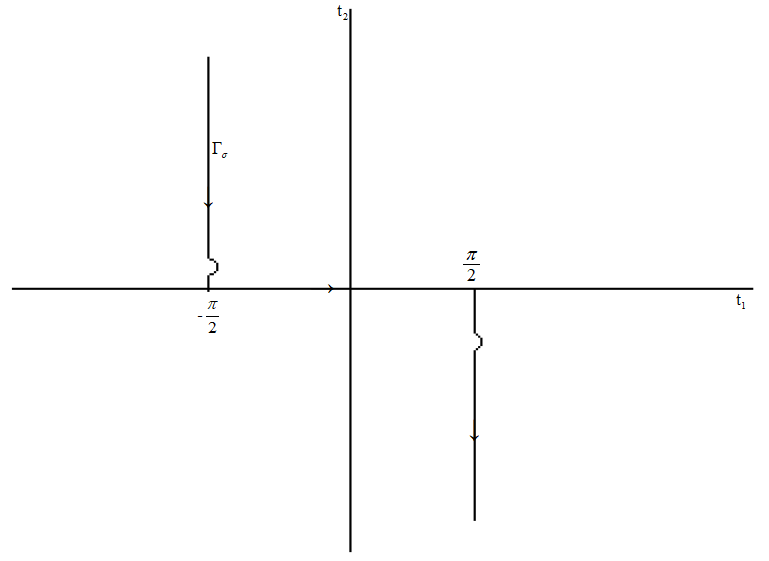
\includegraphics[width=0.8\textwidth,height=0.5\textwidth]{./graphic/transfor2.png}
	\caption{Transform from $P_\sigma$ in the $\xi$-plane to $\Ga_\sigma$ in the t-plane}\label{figure_trans}
\end{figure}

Similarly, if $\sigma$ small enough, we can taking the shift transformation of t and use cauchy integral theorem.
Therefore, the proof of this lemma can be completed  by the same method as employed in the lemma \ref{es_dgreen}. Here we omit the details.
\finproof

In the following we will use the weighted norm $\|u\|_{H^1(D)}=(\|\na \phi\|_{L^2(D)}^2+d_D^{-2}\|\phi\|_{L^2(D)}^2)^{1/2}$ be the weighted $H^1(D)$ norm
and
$\|v\|_{H^{1/2}(\Ga)}=(d_D^{-1}\|v\|_{L^2(\Ga)}^2+|v|_{\frac 12,\Ga}^2)^{1/2}$ be the weighted $H^{1/2}(\Ga)$ norm,
where $d_D$ is the diameter of $D$ and
\ben
|v|_{\frac 12,\Ga}=\left(\int_\Ga\int_\Ga\frac{|v(x)-v(y)|^2}{|x-y|^2}ds(x)ds(y)\right)^{1/2}.
\een
By scaling argument and trace theorem we know that there exists a constant $C>0$ independent of $d_D$ such that for any $\phi\in C^1(\bar{D})^2$ \cite[corollary 3.1]{RTMhalf_aco},
\be\label{q0}
\|\phi\|_{H^{1/2}(\Ga_D)}+\|\sigma(\phi)\cdot\nu\|_{H^{-1/2}(\Ga_D)}\le C\max_{x\in D}(|\phi(x)|+d_D|\na\phi(x)|) 
\ee
We finish this section by introducing  some results on foward scattering problem which will be discussed briefly in the Appendix of this paper. 
\begin{thm} \label{elastic_eq2}
	Let $g \in H^{1/2}(\Ga_D)$, then the scattering problem of elastic equation in the half space
	\be
	\Delta_e u + \omega^2 u =0 \qquad\mbox{\rm in } \R^2_+\bks \bar{D}, \label{elas_1}\ \ \
	\\ u= g \ \ \ \ \mbox{\rm on } \Ga_D, \label{elas_bd} \\
	\sigma(u)e_2=0 \ \ \ \ \mbox{\rm on} \Ga_0, \label{elas_b0} \\
	u \ \mbox{satisfies the generalized radiation codition\cite{Guzina2006} such that} \nn \\\label{rc}
	\lim_{r\to\infty}  \int_{S_r^+} (\sigma(N(x,y)e_i)\hat{r})\cdot u(x) - (N(x,y)e_i)\cdot (\sigma(u)\hat{r})ds(x)=0
	\ee
	where $S_r^+:=\{x\in \R^2_+ \ | \ \|x\|=r^2\}$, $\hat{r}=x/r$ and $y\in \R_+^2$. Then the problem (\ref{elas_1})-(\ref{rc})
	admits a unique solution $u \in H^{1}_{\rm loc}(\R^2_+ \backslash \bar D)$. Moreover, for any bounded open set $\mathcal O\subset \R^2_+\bks\bar D$ there exists a constant $C>0$ such that
	\be \label{elas_ineq}
	\|u\|_{H^{1}(\mathcal O)}\le C\|g\|_{H^{-1/2}(\Ga_D)}n
	\ee
\end{thm}
We also give the definition of the Dirichlet-to-Neumann mapping for Elastic scattering problems. For any $g\in H^{1/2}(\Ga_D) $, define $T_h(g)= \sigma(u)\nu\in H^{-1/2}(\Ga_D)$ where  $u$ is the corresponding solution of above equation and also $T_f(g)=\sigma(v)\nu$ where $v$ is the solution of full space scattering proble and their operator norm are denoted by $\|T_h\|$ or $\|T_f\|$in the remainder of this paper. For the sake of convenience, we introduce the following notation:
\be\label{bi_op}
\GG(W,U)=\int_{\Ga_D} [W(x)\cdot \sigma(U(x))\nu- \sigma(W(x))\nu\cdot U(x)]ds(x)
\ee
Using this notation, the integral representation formula of the solution U(x) to the scattering
problem (\ref{elas_1})-(\ref{elas_b0}) reads: $U(x)\cdot q=\GG(U(\cdot),\N(\cdot,x)q)$.

\section{Reverse time migration method }
In this section we introduce RTM method for inverse elastic scattering problems in the half space. Assume that there are $N_s$ sources and $N_r$ receivers uniformly distributed on $\Gamma^d_0$, where $\Gamma^d_0=\{(x_1,x_2)^T\in\Gamma_0:x_1\in[-d,d]\},d>0$ is aperture. We denote by $\Omega$ the sampling domain in which the obstacle is sought. Let $h=dist(\Omega,\Gamma_0)$ be the distance of $\Omega$ to $\Gamma_0$. We assume the obstacle $D\subset\Omega$ and there exist constants $0<c_1<1,c_2>0,c_3>0$ such that
\be\label{convention_2}
|x_1|\leq c_1 d , \ \ |x_1-y_1|\leq c_2 h , \ \
|x_2|\leq c_3 h    \ \ \ \forall x,y \in \Omega
\ee
Before proposing RTM imaging function, we first introduce the point spread function which measures the resolution for finding point source\cite{ammari2013mathematical}. In \cite{RTMhalf_aco}, the point spread function has been defined in the case of acoustic wave. We now define a similar elastic point spread function $\J(z,y)$, a $\mathbb{C}^{2\times2}$ matrix, which back-propagate the conjugated data $\overline{N(x,y)}$ as the Dirichlet boundary condition. Thus, for any $z,y \in \R_+^2$
\be\nn\hspace{-1cm}
\J_{ij}(z,y):=e_i\cdot \J(z,y) e_j&=&\int_{\Gamma_0} \ \sigma_x(\D(x,y)e_i)e_2\cdot\overline{\N(x,y)}e_j ds(x) \\ \label{fullpsf}
&=&\int_\R \ \sigma_x(\D(x_1,0;z_1,z_2)e_i)e_2\cdot\overline{\N(x_1,0;y_1,y_2)}e_j dx_1
\ee
The estimate in lemma \ref{es_dgreen}-\ref{es_ngreen} show that the integral above exists. 
Moreover, we define
\ben
\F(z,y)&=&\frac{1}{2\pi}\int^{k_p}_{-k_p} \  \frac{{\Tp}(\xi)^T \overline{\Np}(\xi)}{\overline{\delta(\xi)}} e^{\i \mu_p (z_2- y_2)+\i(y_1-z_1)\xi} d\xi \\
&+&\frac{1}{2\pi}\int^{k_s}_{-k_s} \  \frac{{\Ts}(\xi)^T \overline{\Ns}(\xi)}{\overline{\delta(\xi)}} e^{\i \mu_s (z_2- y_2)+\i(y_1-z_1)\xi} d\xi
\een
 The following theorem show that $\F(z,y)$ is the main contribution to the point spread funciton when $k_s h\gg1$. Put $n_*=\min\{N|\kappa^{2N-1}<1/c_3,N\in \Z_+ \}$. Then we present some primary results for point spread function, whose proof will be stated in seciton 4.
\begin{thm}\label{thm_psf}
	Let $k_s h>1$. For any $z,y\in\Om$, let $\R(z,y)=\J(z,y)-\F(z,y)$ and it satisfy that
	\be\hspace{-2cm}
	|\R_{ij}(z,y)|+k_s^{-1}|\na_y \R_{ij}(z,y)|\leq \frac{C}{\mu}(\frac{1}{(k_s h)^{\frac{1}{2n^*}}}+k_she^{-k_s h\sqrt{\kappa_R^2-1}}):=\frac{C}{\mu} \epsilon_1(k_s h)
	\ee
	uniformly for $z,y\in\Om$. Here $\kappa_R:=k_R/k_s$ and the constant C may dependent on $k_s d_D$ and $\kappa:=k_p/k_s$, but is independent of $k_s$, $k_p$, h, $d_D$.
\end{thm}

Based on the above argument, we know that $\R(z,y)$ becomes small when z,y move away from $\Gamma_0$. Our goal is to show $\F(z,y)$ has the similar decay to the elastic fundamental solution $\Im\Phi(z,y)$ as $|z-y|\to\infty$.
\begin{lem} \label{festimate1}
	For any $z,y\in \R_+^2$, when $z=y$
	\ben 
	|\Im \F_{ii}(z,y)| \geq \frac{1}{4(\lambda+2\mu)} \ , \ i =1 ,2 \\
	\Im \F_{12}(z,y) = \Im \F_{21}(z,y) =0
	\een
	and for $z\neq y$
	\ben
	|\F_{ij}(z,y)|&\le \frac{C}{\mu}[(k_s|z-y|)^{-1/2})+(k_s|z-y|^{-1})]
	\een
	where constant $C$ is only dependent on $\kappa:=k_p/k_s$.
\end{lem}
By (\ref{q0}), we obtain the following consequence of theorem \ref{thm_psf} and Lemma \ref{festimate1} whcih will be used in the resolution analysis.
\begin{cor}\label{cor_psf}
	There exists a constant C independent of $k_s$, h such that
	\ben\hspace{-2cm}
	\|F(z,\cdot)e_j\|_{H^{1/2}(\Gamma_D)}+	\|\sigma(F(z,\cdot)e_j)\cdot\nu\|_{H^{-1/2}(\Gamma_D)}
	\leq  \frac{C}{\mu}(1+k_s d_D) \\ \hspace{-2cm}
	\|R(z,\cdot)e_j\|_{H^{1/2}(\Gamma_D)}+	\|\sigma(R(z,\cdot)e_j)\cdot\nu\|_{H^{-1/2}(\Gamma_D)}
	\leq  \frac{C}{\mu}(1+k_s d_D) \epsilon_1(k_s h)
	\een
	uniformly for $z\in\Om$, where $d_D$ is the diameter of the obstacle D.	
\end{cor}

Now we consider the finite aperture point spread function $\J_d(z,y)$:
\be
\J^d_{ij}(z,y)=&\int_{-d}^{d} \ \sigma_x(\D(x_1,0;z_1,z_2)e_i)e_2\cdot\overline{\N(x_1,0;z_1,z_2)}e_j dx_1
\ee
Our aim is to estimate the difference $J(z,y)-J_d(z,y)$. It is easy to see that

\be
\frac{(x_1-z_1)^2}{\rho^2}\geq \frac{(1-c_1)^2}{(1-c_1)^2+c_3^2 (h/d)^2}:=m(h/d)\\
\frac{z_2^2}{\rho^2}\leq\frac{c_3^2}{(1-c_1)^2(h/d)+c_3^2 }:=M(h/d)
\ee
where $\rho=\sqrt{(x_1-z_1)^2+z_2^2}$ and $z\in\Omega,x\in \Gamma_0\bks(-d,d)$.
In the sebsequent discussions, we assume $m(h/d)>(1+\kappa)^2/4$, $M(h/d)<\kappa^2/4$.
\begin{thm} \label{ap_psf}
	For $k_s h\geq 1$ and $z,y\in\Omega$, we have
	\be 
	|\J(z,y)-\J_d(z,y)|+k_s^{-1}|\nabla_y(\J(z,y)-\J_d(z,y))|\\
	\leq \frac{C}{\mu} ((\frac{h}{d})^{2}+\frac{(k_s h)^{1/2}}{ e^{k_s h\sqrt{\kappa_R^2-1}}}(\frac{h}{d})^{1/2}):=\frac{C}{\mu} \epsilon_2(k_s h,h/d)
	\ee
	where the constant C is only dependent on $\kappa$.
\end{thm}
\debproof
By lemma \ref{es_ngreen}, lemma \ref{es_dgreen} and $k_s h\geq 1$, we have
\ben
\Bigg| \int_{d}^{\infty} (T_D(x_1,0;z_1,z_2))^T\overline{N(x_1,0;y_1,y_2)}dx_1
\Bigg| \\
\leq
\frac{C}{\mu}\int_{d}^{\infty}\frac{k_s z_2}{|x-z|}\frac{1}{(k_s|x-z|)^{1/2}}\bigg(
\frac{ y_2}{|x-y|}\frac{1}{(k_s|x-y|)^{1/2}}+e^{-\sqrt{k_R^2-k_s^2}y_2}\bigg) dx_1\\
\leq
\frac{C}{\mu}\int_{(1-c_1)d/h}^{\infty}\frac{1}{(1+t^2)^{3/2}}+\frac{(k_s h)^{1/2}}{(1+t^2)^{3/4}} e^{-\sqrt{k_R^2-k_s^2}h}  dt\\
\leq \frac{C}{\mu} ((\frac{h}{d})^{2}+\frac{(k_s h)^{1/2}}{ e^{\sqrt{k_R^2-k_s^2}h}}(\frac{h}{d})^{1/2})
\een
Here we have used the first inequeality in (\ref{convention_2}). Similarly, we can prove that the estimate for te integral in $[-\infty,-d]$. This shows the estimate for $J(z,y)-J_d(z,y)$. The estimate for $\nabla_y(J(z,y)-J_d(z,y))$ can be proved similarly.
\finproof
By (\ref{q0}) we obtain the following corollary
\begin{cor}\label{cor_dpsf}
	Let $\R_d(z,y)=\J(z,y)-\J_d(z,y)$. For $k_s h\geq 1$ and $z,y\in\Omega$, there exists a constant C independent of $k_s$, h such that
	\ben\hspace{-2cm}
	\|\R_d (z,\cdot))e_j\|_{H^{1/2}(\Gamma_D)}+	\|\sigma(\R_d (z,\cdot)e_j)\cdot\nu\|_{H^{-1/2}(\Gamma_D)} 
	\leq \frac{C}{\mu} \epsilon_2(k_s h,h/d)(1+k_sd_D)
	\een
	uniformly for $z\in\Om$, where $d_D$ is the diameter of the obstacle D.	
\end{cor}

Motivated by the above discussion, we introduce the following imaging function:
\begin{alg}{\sc (Reverse time migration algorithm)}\label{alg_rtm}\\
	Given the data $u_k^s(x_r,x_s)$, $k=1,2$ which is the measurement of the scattered field at $x_r$ when the source is emitted at $x_s$ along the  polarized direction $e_k$, $s=1,\dots, N_s$ and $r=1,\dots,N_r$. 
\be\label{cor1} \hspace{-2cm}
I_d(z)=\Im\sum_{k=1}^{2}\left\{\frac{|\Gamma_0^d|}{N_s}\sum^{N_s}_{s=1}\sum_{i=1}^{2}[\sigma_{x_s}(\D(x_s,z)e_i)e_2\cdot e_k][v_k(z,x_s)\cdot e_i]\right\}. \ \ z\in \Omega
\ee
where $v_k(z,x_s)$ satisfy the following scattering elastic equation:
\ben
\Delta_e v_k(z,x_s) + \omega^2 v_k(z,x_s) =0 \qquad\mbox{\rm in } \R^2_+ \\
v_k(z,x_s)=\frac{|\Ga_0^d|}{N_r}\sum_{r=1}^{N_r}\overline{u^s_k(x_r,x_s)}\delta_{x_r}(z) \ \ \ \ \mbox{\rm on} \Ga_0
\een
By letting $N_s,N_r\to\infty$, we know that (\ref{cor1}) can be viewed as an approximation of the following continuous integral:
\ben\hspace{-3cm}
\hat{I}_d(z)=\Im\sum_{k=1}^{2}\int_{\Gamma_0^d}\int_{\Gamma_0^d}\sum_{i=1}^{2}[\sigma_{x_s}(\D(x_s,z)e_i)e_2\cdot e_k]
[\sigma_{x_r}(\D(x_r,z)e_i)e_2\cdot\overline{u^s_k(x_r,x_s)}]ds(x_r)ds(x_s)
\een
where $z\in\Om$.
\end{alg}

Now, We turn to  study the resolution of the function $\hat{I}_d(z)$. To do this, we first show the difference between the half space scattering solution and the full space sacttering solution is small if the sactterer is far away from the boundary $\Ga_0$.
\begin{thm}\label{diff_solu}
	Let $g\in H^{1/2}(\Ga_D)$ and $\u_1,\u_2$ be the scattering solution of following problems:
	\be\label{elas_r1}
	\Delta_e \u_1 + \omega^2 \u_1=0 \qquad\mbox{\rm in } \R^2_+\bks \bar{D}\\
	\u_1= g \ \ \ \ \mbox{\rm on } \Ga_D  \label{elas_rbd}\\
	\sigma(\u_1)e_2=0 \ \ \ \ \mbox{\rm on} \Ga_0 \label{elas_rb0}
	\ee
	and
	\be {\label{elas_r2}}
	\Delta_e \u_2 + \omega^2 \u_2=0 \qquad\mbox{\rm in } \R^2\bks \bar{D}\\
	\u_2 = g \ \ \ \ \mbox{\rm on } \Ga_D  \label{elas_rbd2}
	\ee
	Then there exits a constant C independant of $k_s$, $k_p$, such that
	\be\hspace{-2.3cm}
	\|\sigma_x(\u_1-\u_2)\nu\|_{H^{-1/2}(\Gamma_D)}
	\leq \frac{C}{\mu}(1+\|T_f\|)(1+\|T_h\|)(1+k_s d_D)^2\epsilon_1(k_s h)\|g\|_{ H^{1/2}(\Ga_D)}
	\ee
\end{thm}
Theorem \ref{diff_solu} also will be proved in the appendix of this paper. The following theorem is the main result of resolution analysis.
\begin{thm}\label{resolution1}
	For any $z\in\Omega$, let $\Psi(y,z)\in\C^{2\times2}$ be the radiation solution of the problem:
	\ben
	& & \Delta_e \Psi(y,z)e_i + \omega^2\Psi e_i= 0 \ \ \ \ \mbox{in }\R_+^2\bks \bar{D} \ \ \ i=1,2 \\
	& &\Psi(y,z)= -\overline{\F(z,y)} \ \ \ \ \ \ \ \mbox{on} \ \Ga_D  \\ 
	\een
	Then, we have
	\be\hspace{-1cm}
	\hat{I}_d(z)=\Im\int_{\Gamma_D}\sum_{i=1}^2[\sigma_y (\overline{(\F(z,y)}+\Psi(y,z))e_i)\cdot \overline{\F(z,y)}e_i]ds(y)+\W_{\hat{I}}(z)
	\ee
	where $|\W_{\hat{I}}(z)|\leq \frac{C}{\mu}(1+\|T_f\|)(1+\|T_h\|)(1+k_s d_D)^4(\epsilon_1(k_s h)+\epsilon_2(k_s h,h/d))$ uniformly for z in $\Om$.
\end{thm}
\debproof
Denote by $v_k(z,x_s)$ the field back-propagating from $\overline{\u^s_k(x_r,x_s)}$ on $\Ga_d$ where $\u^s_k(x,x_s)+N(x,x_s)e_k=0$.
From (\ref{fullpsf}) and (\ref{bi_op}), we get for any $z\in\Omega$,
\ben\hspace{-1cm}
v_k(z,x_s)\cdot e_i&=&\int_{\Gamma_0^d}\sigma_{x_r}(\D(x_r,z)e_i)e_2\cdot\overline{\u^s_k(x_r,x_s)}ds(x_r) \\
&=&\sum_{j=1}\int_{\Gamma_0^d}e_j^T\sigma_{x_r}(\D(x_r,z)e_i)e_2\GG(\overline{\u^s_k(\cdot,x_s)},\N(\cdot,x_r)e_j)ds(x_r)\\
&=&\GG(\overline{\u^s_k(\cdot,x_s)},\sum_{j=1}\int_{\Gamma_0^d}e_j^T\sigma_{x_r}(\D(x_r,z)e_i)e_2\N(\cdot,x_r)e_j ds(x_r))\\
&=&\GG(\overline{\u^s_k(\cdot,x_s)},\J_d(z,\cdot)^Te_i)
\een
By the definition of the imaging function $\hat{I}_d(z)$, we have
\be\hspace{-1cm}
\hat{I}_d(z)&=&\Im\sum_{k=1}^{2}\int_{\Gamma_0^d}\sum_{i=1}^2(e_k\cdot
\sigma_{x_s}(\D(x_s,z)e_i)e_2)( v_k(z,x_s)\cdot e_i) ds(x_s)\\
&=& \Im\sum_{k=1}^{2}\int_{\Gamma_0^d}\mathbf{tr}[( v_k(z,x_s)\cdot e_i)(e_k^T
\sigma_{x_s}(\D(x_s,z)e_j)e_2)]_{ij} ds(x_s)\\
&=&\Im\mathbf{tr}[\GG(\sum_{k=1}^{2}\int_{\Gamma_0^d}\overline{\u^s_k(\cdot,x_s)}e_k^T
\sigma_{x_s}(\D(x_s,z)e_j)e_2 ds(x_s),\J_d(z,\cdot)^Te_i)]_{ij}\\ \label{resolu_1}
&=&\Im\mathbf{tr}[\GG(\W(\cdot,z)e_j,\J_d(z,\cdot)^Te_i)]_{ij}
\ee
where
\be
\W(y,z)e_j= \sum_{k=1}^{2}\int_{\Gamma_0^d}\overline{\u^s_k(\cdot,x_s)}e_k^T
\sigma_{x_s}(\D(x_s,z)e_j)e_2 ds(x_s)
\ee
Therefore, $\overline{\W(y,z)}e_j$ can be viewed as the weighted superposition of $u^s_k(y,x_s)$.
On the boundary of the obstacle $\Gamma_D$, we have
\ben
\overline{\W(y,z)}e_j&=&\sum_{k=1}^{2}\int_{\Gamma_0^d}\u^s_k(y,x_s)e_k^T
\sigma_{x_s}(\overline{\D(x_s,z)}e_j)e_2 ds(x_s) \\
&=&\sum_{k=1}^{2}\int_{\Gamma_0^d}-\N(y,x_s)e_k e_k^T
\sigma_{x_s}(\overline{\D(x_s,z)}e_j)e_2 ds(x_s)\\
&=&-\overline{\J_d^T(z,y)}e_j
\een
Moreover, $\sigma_y(\overline{\W(y,z)}e_j)e_2=0$ on $\Gamma_0$ since $\sigma_y(\overline{u^s_k(y,x_s)})e_2=0$ on $\Gamma_0$. Let $\W_d(y,z)$ be the scattering solution of the problem
\be
& & \Delta_e \W_d(y,z)e_j + \omega^2 \W_d(y,z)e_j= 0 \ \ \ \ \mbox{in }\R_+^2\bks \bar{D}\\
& &\W_d(y,z)= \overline{\F(z,y)}-\overline{\J_d^T(z,y)} \ \ \mbox{on} \ \Ga_D  \\ 
& & \sigma_y(\W_d(y,z)e_j)e_2=0 \ \ \mbox{on} \ \Ga_0
\ee
By theorem \ref{elastic_eq2} and Corollaries \ref{cor_psf}-\ref{cor_dpsf} we have
\be\label{W_ineq}
\|\sigma_y(\W_d(y,z)e_j)e\nu\|_{H^{-1/2}(\Gamma_D)}&\leq& 	\|T_h\|\|\F(z,\cdot)e_j-\J_d^T(z,\cdot)e_j\|_{H^{1/2}(\Gamma_D)}
\ee
Let $ \V(y,z):=\overline{ \W(y,z)}-\W_d(y,z)-\Psi(y,z)$. Since $\overline{ \W(y,z)}-\W_d(y,z)$ satisfy the half-space scattering problem \ref{elas_r1} with $g(y)=-\overline{\F(z,y)}$, by Theorem \ref{diff_solu}, we have
\be
\|\sigma_y(\V(y,z)e_j)\nu\|_{H^{1/2}(\Gamma_D)}\\ \hspace{-0.5cm}
\leq \frac{C}{\mu}(1+\|T_f\|)(1+\|T_h\|)(1+k_s d_D)^2\epsilon_1(k_s h)\|\F(z,\cdot)e_j\|_{H^{1/2}(\Gamma_D)}
\ee
Now we substitute $\overline{ \W(y,z)}=\V(y,z)+\W_d(y,z)+\Psi(y,z)$ into (\ref{resolu_1}) to obtain
\be\hspace{-1.5cm}\label{I_d}
\hat{I}_d(z)=\Im\mathbf{tr}[\GG(\overline{\Psi(\cdot,z)}e_j,\J_d(z,\cdot)^Te_i)]_{ij}+R_{\hat{I}}(z)
\ee
where
\be\hspace{-1.5cm}
R_{\hat{I}}(z)=\Im\mathbf{tr}[\GG(\overline{\V(\cdot,z)}e_j,\J_d(z,\cdot)^Te_i)]_{ij}+\Im\mathbf{tr}[\GG(\overline{\W_d(\cdot,z)}e_j,\J_d(z,\cdot)^Te_i)]_{ij}
\ee
By (\ref{W_ineq}) and Corollaries \ref{cor_psf}-\ref{cor_dpsf} it is easy to see that
\be\hspace{-1.5cm}
|R_{\hat{I}}(z)|\leq \frac{C}{\mu}(1+\|T_f\|)(1+\|T_h\|)(1+k_s d_D)^4(\epsilon_1(k_s h)+\epsilon_2(k_s h,h/d))
\ee
Finally, by (\ref{I_d}) and $\Psi(y,z)= -\overline{\F(z,y)}$ on $\Ga_D$
\ben\hspace{-2cm}
\hat{I}_d(z)=\Im\mathbf{tr}[\GG(\overline{\Psi(\cdot,z)}e_j,\F(z,\cdot)e_i)]_{ij}+\Im\mathbf{tr}[\GG(\overline{\Psi(\cdot,z)}e_j,(\J^T_d(z,y)-\F(z,y))e_i)]_{ij}+R_{\hat{I}}(z) \\ \hspace{-1cm}
=\Im\sum_{i=1}^2\int_{\Gamma_D}[\sigma_y (\overline{(\F(z,y)}+\Psi(y,z))e_i)\cdot \overline{\F(z,y)}e_i]ds(y)+w_{\hat{I}}(z)+R_{\hat{I}}(z)
\een
By Corollaries \ref{cor_psf}-\ref{cor_dpsf} we have
\be
|w_{\hat{I}}(z)|\leq \frac{C}{\mu}(1+\|T_h\|)(1+k_s d_D)^2(\epsilon_1(k_s h)+\epsilon_2(k_s h,h/d))
\ee
\finproof
By (\ref{F_p})-(\ref{F_s}) we know that for any fixed $z\in\Om$, $\overline{\F(z,\cdot)}$ satisfies the Elastic wave equation. Thus $\Psi(y,z)$ can be viewed as the scattering solution of the Elastic equation with the
incident wave $\overline{\F(z,\cdot)}$. By lemma \ref{festimate1} we konw that $\overline{\F(z,\cdot)}$ decays as $|y-z|$ becomes large. Therefore the imaging function $\hat{I}_d(z)$ becomes small when z moves away from the
boundary $\Ga_D$ outside the scatterer $D$ if $k_s h \gg 1$ and $d\gg h$.

To understand the behavior of the imaging fuction when $z$ is close to the boundary of the scatterer, we extend the concept of the scattering coefficient fo incident plane waves\cite{RTMhalf_aco}.
\begin{definition}\label{scarr_con}
	For any unit vector $d\in \R^2$, let $u^i_p =d e^{\i k_p x\cdot d}$ or $u^i_s= d^\perp e^{\i k_s x\cdot d}$ be the incident wave and $u^s_\alpha = u^s_\alpha(x;d)$ be the corresponding radiation solution of the Navier equation:
	\be
	u^s_\alpha + \om^2u^s_\alpha = 0\ \ \mbox{in} \ \  \R^2\bks\bar{D} \\
	u^s_\alpha =-u^i_\alpha \ \ \mbox{on} \ \ \pa D 
	\ee
	The scattering coecient R(x;d) for $x\in\pa D$ is defined by the relation
	\ben
	\sigma(u^s_\alpha+u^i_\alpha)\cdot \nu= \i k_\alpha R_\alpha(x;d)e^{\i k_\alpha x\cdot d}  \ \ \ \mbox{on}\ \ \pa D
	\een
	where $\alpha=p,s$, $d=(d^1,d^2)^T$ is unit vectors, $d^\perp=(d^2,-d^1)^T$ .
\end{definition}
In the case of high frequency approximation, the scattering coecient can be approximated by
\ben
R_\alpha(x;d)=\left\{ \begin{array}{ll}
	RF_\alpha(d;\nu(x))    \ \  \  \mbox{if} \ \ x \in \pa D^{-}_d=\{x\in \pa D, \nu(x)\cdot d<0\},\\ 
	0 \ \ \ \ \ \ \ \  \ \ \ \ \ \ \  \ \ \ \mbox{if} \ \ x \in \pa D^{+}_d=\{x\in \pa D, \nu(x)\cdot d\geq0\}.
\end{array} \right.
\een
Now we consider the physical interpretation of the imaging function $\hat{I}_d(z)$ when $z\in\Ga_D$. By (\ref{F_p}) and (\ref{F_s}), we have
\ben\hspace{-2cm}
\overline{F(z,y)}=\i\int_{0}^{\pi}A_p(\theta)\eta_\theta e^{\i k_p (y-z)\cdot \eta_\theta}+A_s(\theta)\eta_\theta^\perp e^{\i k_s (y-z)\cdot \eta_\theta}d\theta, \ \ \ \ \eta_\theta:=(\cos\theta,\sin\theta)^T
\een
where 
\ben
A_p(\theta)=\frac{ k_s^2k_p^3 \mu_s(k_p\cos\theta)\sin\theta}{2\pi\mu\gamma(k_p\cos\theta)\delta(k_p\cos\theta)}(\cos\theta,\sin\theta)
\een
and
\ben\hspace{-2cm}
A_s(\theta)=\left\{ \begin{array}{ll}
	\frac{ k_s^5\mu_p(k_s\cos\theta)\sin\theta}{2\pi\mu\gamma(k_s\cos\theta)\delta(k_s\cos\theta)}(\sin\theta,-\cos\theta) \ \ \ \ \ \ \ \ \ \theta\in(\arccos(k_p),\arccos(-k_p)) \\
	\frac{ k_s^5(1-4\cos^2\theta)\overline{\mu_p(k_s\cos\theta)}\sin\theta}{2\pi\overline{\gamma(k_s\cos\theta)}\delta(k_s\cos\theta)}(\sin\theta,-\cos\theta) \ \ \theta\in(0,\pi)\bks[\arccos(k_p),\arccos(-k_p)]
\end{array}\right.
\een
Let y(s) be the arc length parametrization of the boundry $\Ga_D$ and $y_{\pm}(\eta_\theta)=y(s_{\pm})$ be the pionts such that $\nu(y(s_{\pm}))=\pm\eta_\theta$. By the same procedure used in \cite[p11,12]{RTMhalf_aco}, we can obtain
\ben\hspace{-1cm}
\hat{I}_d(z)&\approx&\sqrt{8\pi k_p}\Im\mathbf{tr} \int_{0}^{\pi}((\lambda+2\mu)A_p(\theta)\eta_\theta e^{\i k_p (y_-(\eta_\theta)-z)\cdot \eta_\theta-\i\frac{\pi}{4}})^T\frac{\overline{F(z,y_-(\eta_\theta))}}{\sqrt{\vartheta(y_-(\eta_\theta))}}d\theta \\
&+&\sqrt{8\pi k_s}\Im\mathbf{tr} \int_{0}^{\pi}(\mu A_s(\theta)\eta_\theta^\perp e^{\i k_s (y_-(\eta_\theta)-z)\cdot \eta_\theta-\i\frac{\pi}{4}})^T\frac{\overline{F(z,y_-(\eta_\theta))}}{\sqrt{\vartheta(y_-(\eta_\theta))}}d\theta
\een
Now for z in the part of $\Ga_D$ which is back to $\Ga_0$, ie $\nu(z)\cdot\eta_\theta>0$ for any $\theta\in[0,\pi]$, we know that z and $y_{-}(\eta_\theta)$ are far away and thus $\hat{I}_d(z)\approx0$. By above formula and lemma \ref{festimate1}, we can explain that one cannot image the back part of the obstacle with only the data collected on $\Ga_0$. This confirmed in our numerical examples.
\section{Analysit of point spread function}

In this section we give the proof of theorem \ref{thm_psf} and lemma \ref{festimate1} which depend on several lemmas that follow.
Without loss of generality. we assume $z_1-y_1\geq0$ in the sebsequent. Otherwise, we can take substitution $\xi=-\xi$.

We split the spectral terms into components associated with pressure and shearing waves.
\ben
\hat{\D}=\hat{\D^p}+\hat{\D^s} \ \ \ \ \ \ \ \ \ \
\hat{\N}=\hat{\N^p}+\hat{\N^s} \ \ \,
\een
and we define
\be\hspace{-1cm}
\J^{\alpha\eta}_{ij}(z,y)&=&\int_{\Gamma_0} \ \sigma_x(\D^\alpha(x,y)e_i)e_2\cdot\overline{\N^{\eta}(x,y)}d)e_j ds(x),
\ \ \ \  \alpha,\eta\in\{s,p\}
\ee
It's esay to see
\ben
\J(z,y)=\sum_{\alpha=p,s}^{\eta=p,s} \ \J^{\alpha\eta}(z,y)
\een
In order to analysis the PSF, loss is assumed in the medium that $k_{\alpha,\ep}:=k_\alpha(1+\i\ep)$. For $\alpha,\beta\in \{s,p\}$, define $b_{\alpha\beta}=k_s$ only if $\alpha=\beta=s$ , or otherwise $b_{\alpha\beta}=k_p$. Then by Parseval identity, we carry out
\ben\hspace{-1.5cm}
\J^{\alpha\beta}(z,y)&=&\lim_{\ep\to 0^+} \ \frac{1}{2\pi} \int_R \  \frac{{\Ta^{\ep}}(\xi)^T \overline{\Nb^{\ep}}(\xi)}{\overline{\delta^{\ep}(\xi)}} e^{\i (\mu_\alpha^{\ep} z_2-\overline{\mu_\beta^{\ep}} y_2)+\i(y_1-z_1)\xi} d\xi\\
&=& \frac{1}{2\pi}\int^{b_{\alpha\beta}}_{-b_{\alpha\beta}} \  \frac{{\Ta}(\xi)^T \overline{\Nb}(\xi)}{\overline{\delta(\xi)}} e^{\i (\mu_\alpha z_2-\overline{\mu_\beta} y_2)+\i(y_1-z_1)\xi} d\xi  \\
&+&\lim_{\ep\to 0^+} \ \frac{1}{2\pi}\int_{R\bks[-b_{\alpha\beta},b_{\alpha\beta}]} \  \frac{{\Ta^{\ep}}(\xi)^T \overline{\Nb^{\ep}}(\xi)}{\overline{\delta^{\ep}(\xi)}} e^{\i (\mu_\alpha^{\ep} z_2-\overline{\mu_\beta^{\ep}} y_2)+\i(y_1-z_1)\xi} d\xi   \\
&:=&\F^{\alpha\beta}(z,y)+\R^{\alpha\beta}(z,y)
\een
By the defination of Cauchy principle value, we can obtian
\ben\hspace{-1.5cm}
\R^{\alpha\beta}(z,y)&=&\frac{1}{2\pi}\int_{[-k_s,k_s]\bks[-b_{\alpha\beta},b_{\alpha\beta}]}+\pv\int_{R\bks[-k_s,k_s]}   \frac{{\Ta}(\xi)^T \overline{\Nb}(\xi)}{\overline{\delta(\xi)}} e^{\i (\mu_\alpha z_2-\overline{\mu_\beta} y_2)+\i(y_1-z_1)\xi} d\xi \\
&-&\frac{\i}{2}\Big(\frac{{\Ta}(k_R)^T \overline{\Nb}(k_R)}{\overline{\delta'(k_R)}}e^{\i(y_1-z_1)k_R}-\frac{{\Ta}(-k_R)^T \overline{\Nb}(-k_R)}{\overline{\delta'(-k_R)}}e^{-\i(y_1-z_1)k_R}\Big)e^{-\sqrt{k_R^2-k_\alpha^2}z_2-\sqrt{k_R^2-k_\beta^2}y_2}
\\
&:=&\R_1^{\alpha\beta}(z,y)+\R_2^{\alpha\beta}(z,y)+\R_3^{\alpha\beta}(z,y)
\een
\begin{lem}\label{pv_term}
Let $d=(\kappa_R-1)/2$, then we have
\ben
|\pv \int_{1}^{\infty}\frac{k_s^4 g(t)}{\delta(k_s t)}|\leq C\Big( \int_{1}^{\infty}|g(t)|dt+ \max_{t\in[\kappa_R-d,\kappa_R+d]}(|g(t)|+|g'(t)|)\Big)
\een
where $\kappa_R = k_R/k_s$ and C only depend on $\kappa$.
\end{lem}
\debproof
Since $\delta(k_s t)$ has a zero at $\kappa_R$ of order one, we can choose $\sigma>0$ small enough such that 
\be\label{de_eq}
0<C_1\leq\frac{\delta'(k_s t)}{k_s^3}<C_2, \ \ \ \frac{\delta''(k_s t)}{k_s^2}<C_2
\ee
for any $t\in I_1=(\kappa_R-\sigma,\kappa_R+\sigma)$ .
Let $\delta_1(t)=\frac{\delta(k_s t)}{k_s^4 (t-\kappa_R)}$ and $I_2=(1,\infty)\bks I_1$ we have
\ben \hspace{-1.5cm}
|\pv \int_{{1}^{\infty}}\frac{k_s^4 g(t)}{\delta(k_s t)}|\leq
|\pv\int_{I_1}\frac{k_s^4 g(t)}{\delta(k_s t)}dt|+|\int_{I_2}\frac{k_s^4 g(t)}{\delta(k_s t)}dt|\\  \hspace{-2cm}
\leq |\int_{I_1}\frac{g(t)\delta_1(t)^{-1}-g(\kappa_R)\delta_1(\kappa_R)^{-1}}{t-\kappa_R}+\pv\int_{I_1}\frac{g(\kappa_R)\delta_1(\kappa_R)^{-1}}{t-\kappa_R}|+\max_{t\in I_2}\frac{k_s^4}{\delta(k_s t)}\int_{I_2}|g(t)|dt\\ \hspace{-2cm}
\leq \max_{t\in I_1}|\big(\frac{g(t)}{\delta_1(t)}\big)'|
+C\frac{k_s^4}{\delta(k_s t)}\int_{I_2}|g(t)|dt
\een
By the mean value theorem and \ref{de_eq}, for any $t\in (1,2\kappa_R-1)$ we have
\ben
(\frac{g(t)}{\delta_1(t)})'=\frac{g'(t)\delta'(k_s t_1)k_s^5-g(t)\delta''(k_s t_2)k_s^6/2}{\delta'(k_s t_1)} \ \ \ t_1,t_2\in [\kappa_R,t] \ \mbox{or} \ [t,\kappa_R] \\
\leq C\max_{t\in I_1}(|g(t)|+|g'(t)|)
\een
This completes the proof.
\finproof

\begin{lem}\label{medi_term}
	Let $f(t)$ be a complex valued function in $(\kappa,\infty)$ and satisfy that $|f(t)|<C(1+t^k), k\in \Z_+$. Then for $\rho>1$ we have
	\ben
	|\int_{\kappa}^{1}|f(t)e^{-\rho \sqrt{t^2-\kappa^2}}d\xi|
	\leq C\frac{1}{\rho} \\
	|\int_{1}^{\infty}|f(t)e^{-\rho \sqrt{t^2-1}}d\xi|
	\leq C\frac{1}{\rho}
	\een  
\end{lem}
\debproof
It is simple to see that
\ben
|\int_{\kappa}^{1}|f(t)e^{-\rho \sqrt{(t^2-\kappa^2)}}dt|\leq C \int_{\kappa}^{1}(1+t^k)e^{-\rho \sqrt{t^2-\kappa^2}}dt \\
\leq C\int_{0}^{\sqrt{(1-\kappa^2)}}\frac{t}{\sqrt{t^2+\kappa^2}}e^{-\rho t}dt \leq C \frac{1}{\rho}
\een
and
\ben
|\int_{1}^{\infty}|f(t)e^{-\rho \sqrt{t^2-1}}dt|\leq C \int_{1}^{\infty}(1+t^k)e^{-\rho \sqrt{t^2-1}}dt \\
\leq C\int_{0}^{\infty}\frac{(1+(t^2+1)^{k/2})t}{\sqrt{t^2+1}}e^{-\rho t}dt \leq C \frac{1}{\rho}
\een
This completes the proof.
\finproof

\begin{lem}\label{cross_term}
	For $0<\kappa<1$, let $F(\lambda)=\int_{0}^{\kappa}f(t)e^{\i\lambda(\sqrt{1-t^2}-\tau\sqrt{\kappa^2-t^2}+\alpha t)}dt$, where $\tau\geq c_0>0$ and $\alpha\in\R$, then we have
	\ben
	|F(\lambda)|\leq C(\kappa) \lambda^{-\frac{1}{2N_*}} \Big[|f(\kappa)|+\int_{0}^{\kappa}|f'(t)|dt\Big]
	\een
	where $N_*=\min\{N|\kappa^{2N-1}<c_0,N\in \Z_+ \}$.
\end{lem}
\debproof
Put $\phi(t)=-\sqrt{1-t^2}$ and $\psi(t,\tau)=\tau\kappa\phi(t/\kappa)-\phi(t)+\alpha t$. For easy of notations, we denote the $n$-th partial derivative of $g(t)$ with respect to $t$ by $g^{(n)}(t)$. Then, it is to see that, for $n>1$
\ben
\psi^{(n)}(t,\tau)=\frac{\tau}{\kappa^{n-1}}\phi^{(n)}(\frac{t}{\kappa})-\phi^{(n)}(t)
\een
A standard computation show that
\ben
\phi^{(1)}(t)=\frac{t}{\sqrt{1-t^2}}  \ \ \
\phi^{(2)}(t)=\frac{1}{(1-t^2)^{3/2}}
\een
Moreover, for $n\geq3$, we have
\be
\phi^{(n)}(t)=\frac{p_n(t)}{(1-t^2)^{n-1/2}}
\ee
where $p_n=\sum_{0}^{n-2}a^n_{k}t^k$ is a $(n-2)$-th polynomial such that its  coefficients satisfy the following recursion formula:
\ben
a^{n+1}_{n-1}=(n+1)a^n_{n-2}, \ \ \ a^{n+1}_{n-2}=(n+2)a^n_{n-3} \\
a^{n+1}_{k}=(k+1)a^n_{k+1}+(2n-k)a^n_{k-1} \ \ \ \mbox{for} \ 1\leq k\leq n-3 \\
a^{n+1}_{0}=a^n_{1}
\een
Since the polynmial coefficients are all positive, it is obvious that for $n\geq 1$, $\phi^{(n)}(t)$ is a monotone increasing positive function. Using the recursion formula, it follows that
\be \label{value_0}
\phi^{(n)}(0)=\left\{ \begin{array}{ll}
	\ \ \ \ \ \ 	0  \ \ \ \ \ \ \ \ \ \ \  \ \ \ \ \ \  \mbox{n is odd},\\
	(n-1)!!(n-3)!! \ \ \mbox{n is even}.
\end{array} \right.
\ee
where $(2k-1)!!$ is double factorial and $n>3$. We are now in the position to proof the inequality. Since $0<\kappa<1$, obersev that 
\ben
\psi^{(2N_*+1)}(t,\tau)\geq \frac{\tau}{\kappa^{2N_*}}\phi^{(2N_*+1)}(t)-\phi^{(2N_*+1)}(t)>0
\een
Therefore, $\psi^{(2N_*)}(t,\tau)$ is monotone increasing in $[0,\kappa)$. By (\ref{value_0}), we get
\be\hspace{-1.5cm}
\psi^{(2N_*)}(t,\tau)\geq\psi^{(2N_*)}(0,\tau)\geq\psi^{(2N_*)}(0,c_0)=C(2N_*)(\frac{c_0}{\kappa^{2N_*-1}}-1)>0
\ee
The lemma is now a direct consequence of lemma (\ref{van}).
\finproof
Now we are in the position to prove the main theorem of this section.

{\it \bf proof of Theorem \ref{thm_psf}}. By lemma \ref{root_Ga} and expresision (\ref{ngreen}),(\ref{tgreen}), it is easy to see that
\ben\hspace{-2cm}
|e_i\cdot\Na(k_s t)e_j|\leq Ck_s^3(1+t^3),  \ \ |e_i\cdot\Ta(k_s t)e_j|\leq C(1+t^2) \ \ \ \ \ \ \ \ \ \ t\in \R \\ \hspace{-2.5cm}
|(\Ta(k_st)e_i\cdot\overline{\Nb(k_s t)}e_je^{\i k_s(y_1-z_1)t-z_2\sqrt{k_\alpha^2-k_s^2t^2}-y_2\sqrt{k_\beta^2-k_s^2t^2}})'|\leq C k_s he^{-\sqrt{k_R^2-k_s^2}}\ \ \ , t\in (\kappa_R-d,\kappa_R+d) 
\een
Substituting $\xi=k_s t$ into $\R_1^{\alpha\beta}(z,y),\R_2^{\alpha\beta}(z,y),\R_3^{\alpha\beta}(z,y)$, the theorem now follows from lemma \ref{pv_term}, lemma \ref{medi_term} and lemma \ref{cross_term}.
\finproof

To prove the lemma \ref{festimate1}, substitute (\ref{tgreen}) and (\ref{ngreen}) into  $F_{ss}(z,y),F_{pp}(z,y)$, then we have
\be
\hspace{-2cm}\label{F_p}
F^{pp}(z,y)=-\frac{1}{2\pi}\int_{(-k_p,k_p)} \frac{\i k_s^2\mu_s}{\mu\gamma(\xi)\delta(\xi)}
\Bigg(
\begin{array}{cc}
	\xi^2 & -\xi\mu_p \\
	-\xi\mu_p & \mu_p^2
\end{array}		\Bigg)e^{\i\mu_p (z_2-y_2) +\i\xi(y_1-z_1)} \\
\hspace{-2cm}\label{F_s}
F^{ss}(z,y)=-\frac{1}{2\pi}\int_{(-k_p,k_p)} \frac{\i k_s^2\mu_p}{\mu\gamma(\xi)\delta(\xi)}
\Bigg(
\begin{array}{cc}
	\mu_s^2 & \xi\mu_s \\
	\xi\mu_s & \xi^2
\end{array}		\Bigg)e^{\i\mu_s (z_2-y_2) +\i\xi(y_1-z_1)} \\ \nn
-\frac{1}{2\pi}\int_{(-k_s,k_s)\bks(-k_p,k_p)} \frac{\i(k_s^2-4\xi^2)\mu_p}{\mu\gamma(\xi)\overline{\delta(\xi)}}
\Bigg(
\begin{array}{cc}
	\mu_s^2 & \xi\mu_s \\
	\xi\mu_s & \xi^2
\end{array}		\Bigg)e^{\i\mu_s (z_2-y_2) +\i\xi(y_1-z_1)} \\ \nn
:=F^{ss1}(z,y)+F^{ss2}(z,y)
\ee

{\it \bf proof of Lemma \ref{festimate1}}.
We only proof the case of $i=j=1$, the other ones are similar.
First, we have $\gamma(\xi)\le k_s^2$, $\delta(\xi)\le k_s^4$ and $\mu_p\le\mu_s$ when $\xi\in(-k_p,k_p)$. Then, if $z=y$
\be
-\Im (F^{pp}_{11}+F^{ss1}_{11})\geq\frac{1}{2\pi\mu}\int_{(-k_p,k_p)} \frac{\mu_p}{k_s^2}d\xi \\ =\frac{k_p^2}{2\pi\mu k_s^2}\int_{0}^{\pi} \sin^2(t) dt= \frac{1}{4(\lambda+2\mu)}
\ee
It's left to proof $-\Im F^{ss2}_{11}>0$. If $\xi\in(-k_s,k_s)\bks(-k_p,k_p)$, $\mu_p=\i\sqrt{\xi^2-k_p^2}$. Substituting it into $F^{ss2}$, we have
\be
\hspace{-1.5cm}
F^{ss2}_{11}=\frac{1}{2\pi\mu}\int_{(-k_s,k_s)\bks(-k_p,k_p)} \frac{\mu_s^2\sqrt{\xi^2-k_p^2}(k_s^2-4\xi^2)}{(\xi^2+\i\mu_s\sqrt{\xi^2-k_p^2})(\beta^2-\i4\xi^2\mu_s\sqrt{\xi^2-k_p^2})} d\xi
\ee
let $\alpha=(\xi^2+\i\mu_s\sqrt{\xi^2-k_p^2})(\beta^2-\i4\xi^2\mu_s\sqrt{\xi^2-k_p^2})$. A simple computation show that $\Im \alpha=k_s^2\mu_s\sqrt{\xi^2-k_p^2}(k_s^2-4\xi^2)$. It is easy to see that
\ben
-\Im F^{ss2}_{11}=\frac{k_s^2}{2\pi\mu}\int_{(-k_s,k_s)\bks(-k_p,k_p)} \frac{\mu_s^3(\xi^2-k_p^2)(k_s^2-\xi^2)^2}{|\alpha|^2} d\xi >0
\een

For $z\neq y$, we denot $y-z=|y-z|(\cos\phi,\sin\phi)^T$ for some $0\le\phi\le2\pi$. Then it is easy to see that
\ben
F^{pp}(z,y)=\frac{1}{\mu}\int_{0}^{\pi} A(\theta,\kappa) e^{\i k_s |z-y| \cos(\theta-\phi)}
\een
The phase function $f(\theta)=\cos(\theta-\phi)$ satisfies $f'(\theta)=-\sin(\theta-\phi),f''(\theta)=-\cos(\theta-\phi)$. For any given $0\le\phi\le2\pi$, we can decompose $[0,\pi]$ into several intervals such that in each either $|f''(\theta)|\ge 1/2$ or $|f'(\theta)|\ge 1/2$ and $f'(\theta)$ is monotonous. The amplitude function $A(\theta,\kappa)$ and their derirates are integrable on $[0,\pi]$. Then the estimate for $F_{pp}(z,y)$ follows by using lemma \ref{van}. The estimation of $F^{ss}(z,y)$ can be proved similarly. This completes the proof.
\finproof






\section{Extensions}
In this section we consider the reconstraction of non-penetrable obstacles with the impedance boundary condition and penetrable obstacle in the half space by the RTM algorithm \ref{alg_rtm}. For non-penetrable obstacles with the impedance boundary condition on the obstacle, the measured data $u^s_k(x_r.x_s)=u_k(x_r,x_s)-N(x_r,x_s)e_k$, $k=1,2$, where $u^s_k(x_r.x_s)$ is the radiation solution of the following problem:
\be\hspace{-2cm}
\Delta_e u^s_k(x) + \omega^2 u^s_k(x) =0 \qquad\mbox{\rm in } \R^2_+\bks \bar{D}, \label{elas_4}\ \ \
\\ \hspace{-2cm} \sigma(u^s_k(x))\nu+\i\eta(x)u^s_k(x)=-(\sigma(N(x,x_s)e_k)\nu+\i\eta(x)N(x,x_s)e_k)\ \ \mbox{\rm on } \Ga_D, \label{elas_bd2} \\ \hspace{-2cm}
\sigma(u^s_k)e_2=0 \ \ \ \ \mbox{\rm on} \ \ \ \Ga_0, \label{elas_b02} 
\ee
By modifying the argument in Theorem \ref{resolution1}, we can show the following result whose proof is omitted.
\begin{thm}\label{resolution2}
	For any $z\in\Omega$, let $\Phi(y,z)\in\C^{2\times2}$ be the radiation solution of the problem:
	\ben
	& & \Delta_e \Psi(y,z)e_j + \omega^2\Psi e_j= 0 \ \ \ \ \mbox{\rm in }\R^2\bks \bar{D}\\
	& &\sigma_y(\Phi(y,z)e_j)\nu+\i\eta(y)\Phi(y,z)e_j= -(\sigma_y(\overline{F(z,y)}e_j)\nu+\i\eta(y)\overline{F(z,y)}e_j )\ \ \mbox{\rm on} \ \Ga_D  \\ 
	\een
	Then, we have
	\ben\hspace{-2.5cm}
	\hat{I}_d(z)=-\Im\int_{\Gamma_D}\sum_{i=1}^2 [((\overline{\F(z,y)}+\Psi(y,z))e_i)\cdot(\sigma_y(\overline{\F(z,y)}e_j)\nu+\i\eta(y)\overline{\F(z,y)}e_i)]ds(y)+W_{\hat{I}}(z)
	\een
	where $|W_{\hat{I}}(z)|\leq C(1+k_s d_D)^4(\epsilon_1(k_s h)+\epsilon_2(k_s h,h/d))$ uniformly for z in $\Om$.
\end{thm}

For the penetrable obstacle , the measured data $u^s_k(x_r.x_s)=u_k(x_r,x_s)-N(x_r,x_s)e_k$, $k=1,2$, where $u^s_k(x_r.x_s)$ is the radiation solution of the following problem:
\be
\Delta_e u^s_k(x) + \omega^2n(x) u^s_k(x) =-\om^2(n(x)-1)N(x,x_s)e_k \qquad\mbox{\rm in } \R^2 \label{elas_5}\ \ \ \\
\sigma(u^s_k)e_2=0 \ \ \ \ \mbox{\rm on} \ \ \ \Ga_0, \label{elas_b03} 
\ee
where $n(x)\in L^{\infty}({\R^2})$ is a positive function which is equel to 1 outside $D$. By modifying the argument in Theorem \ref{resolution1}, the following theorem can be proved.
\begin{thm}\label{resolution3}
	For any $z\in\Omega$, let $\Psi(y,z)\in\C^{2\times2}$ be the radiation solution of the problem:
	\ben
	& & \Delta_e \Psi(y,z)e_j + \omega^2n(y)\Psi e_j= -\omega^2(n(y)-1)\overline{F(z,y)e_j} \ \ \ \ \mbox{\rm in }\R^2
	\een
	Then, we have
	\be\hspace{-2cm}
	\hat{I}_d(z)=-\Im\int_{D}\omega^2(1-n(y))\sum_{i=1}^2 [(\overline{\F(z,y)}+\Psi(y,z))e_i \cdot\overline{F(z,y)}e_i]dy+W_{\hat{I}}(z)
	\ee
	where $|W_{\hat{I}}(z)|\leq C(1+\|n(\cdot)\|_{L^\infty(D)})(1+k_s d_D)^4(\epsilon_1(k_s h)+\epsilon_2(k_s h,h/d))$ uniformly for z in $\Om$.
\end{thm}
\section{Numerical experiments}
In this section we present several numerical examples to show the effectiveness of our
RTM method. To synthesize the scattering data we compute the solution $u^s(x_r; x_s)$ of
the scattering problem by representing the ansatz solution as the single layer potential
with the Green function $N(x; y)$ as the kernel and discretizing the integral equation by
standard $Nystr\ddot{o}m$ methods \cite{colton-kress}. The boundary integral equations on $\Ga_D$ are solved on
a uniform mesh over the boundary with ten points per probe wavelength. The sources
and receivers are both placed on the surface $\Ga_d^0$ with equal-distribution, where d is the
aperture. In all our numerical examples we choose h = 10, d = 50 and \emph{Lam\'{e}} constant $\lambda=1/2$, $\mu=1/4$. The boundaries
of the obstacles used in our numerical experiments are parameterized as follows, 
\ben
\mbox{Circle:}\ \ \ \ &&x_1=\rho\cos(\theta),\ \ x_2=\rho\sin(\theta),\ \ \\
\mbox{Kite:}\ \ \ \ &&x_1=\cos(\theta) + 0.65\cos(2\theta) - 0.65,\ \ x_2=1.5 \sin (\theta),\ \ \\
\mbox{$p$-leaf:}\ \ \ \ &&r(\theta)=1+0.2\cos(p\theta), \\
\mbox{peanut:}\ \ \ \ &&x1 = \cos \theta + 0:2 \cos 3\theta; x2 = \sin \theta + 0:2 \sin 3\theta, \\
\mbox{square:}\ \ \ \ &&x1 = \cos3 \theta + \cos \theta; x2 = \sin3\theta + \sin \theta.
\een
where
$\theta\in[0,2\pi]$. The numerical imaging function is :
\ben\hspace{-2.5cm}
I_d(z)=\Im\sum_{k=1}^{2}\left\{\frac{|\Gamma_0^d|}{N_s}\frac{|\Gamma_0^d|}{N_d}\sum^{N_s}_{s=1}\sum^{N_r}_{r=1}\sum_{i=1}^{2}[\sigma_{x_s}(\D(x_s,z)e_i)e_2\cdot e_k][\sigma_{x_r}(\D(x_r,z)e_i)e_2\cdot\overline{u^s_k(x_r,x_s)}]\right\}
\een

\bigskip
\textbf{Example 1}.
We consider imaging of a Dirichlet, a Neumann, a Robin bounday, and a penetrable obstacle. The imaging domain is $(−2; 2) \times (8; 12)$ with the sampling grid $201 \times 201$ and $N_s = N_r = 401$. The angular frequency is $\om=2\pi$.
 \begin{figure}
 	\centering
 	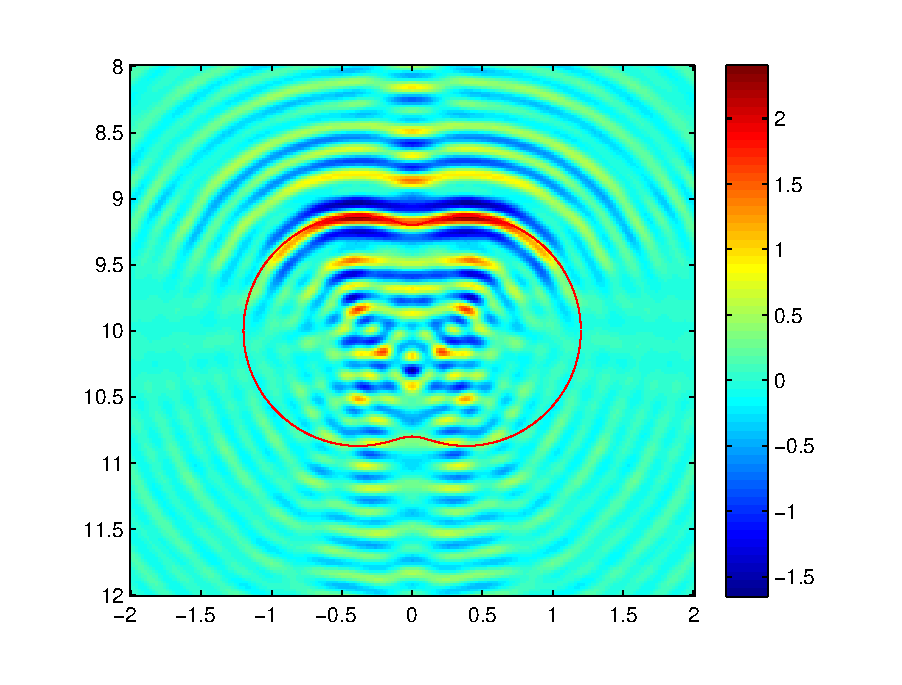
\includegraphics[width=0.24\textwidth]{./graphic/peanut_3pi.eps}
 	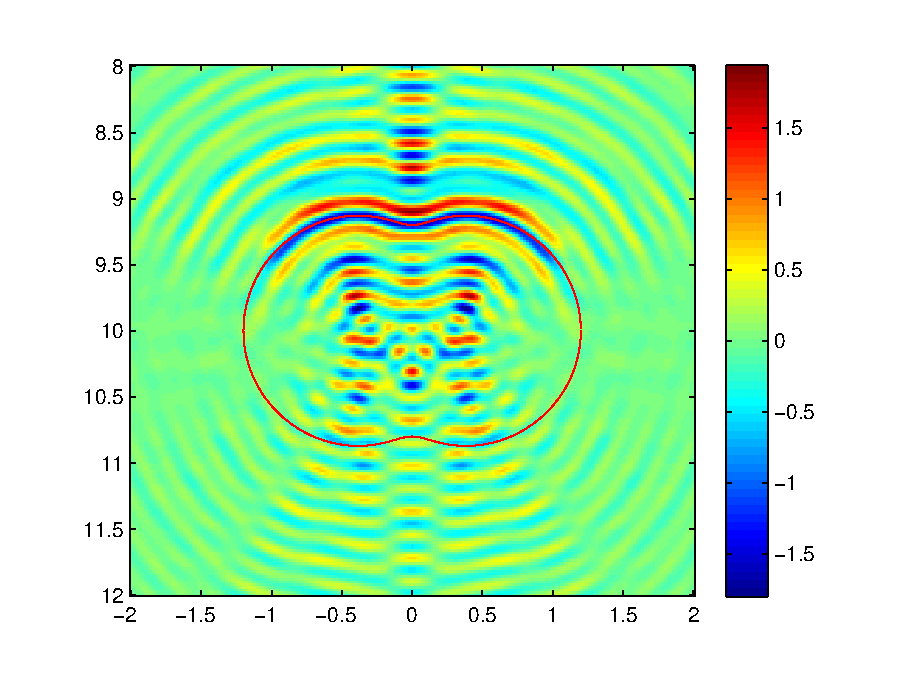
\includegraphics[width=0.24\textwidth]{./graphic/peanut_3pi_neumann.eps}
 	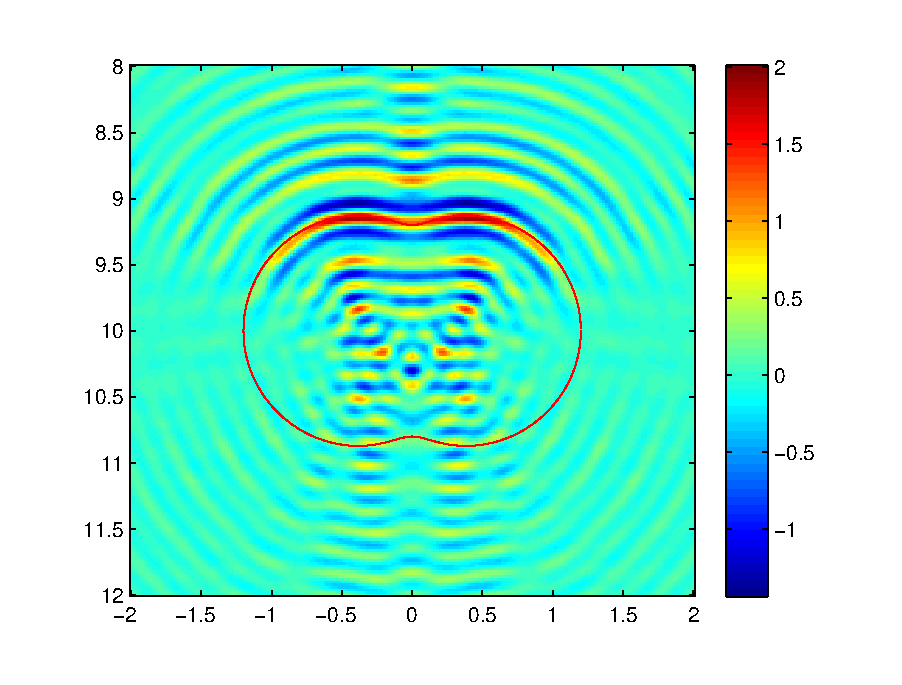
\includegraphics[width=0.24\textwidth]{./graphic/peanut_3pi_impedance_1.eps}
 	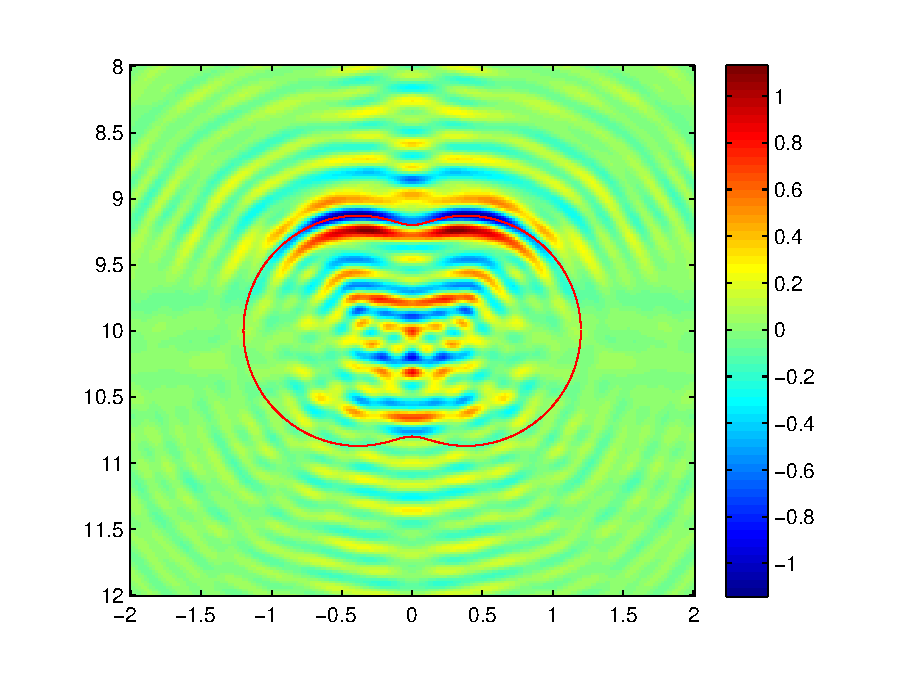
\includegraphics[width=0.24\textwidth]{./graphic/peanut_3pi_transmission.eps}
 	\caption{Example 1: From left to right: imaging results of a Dirichlet, a Neumann, a Robin bounday with impedance $\eta(x)=1$, and a penetrable obstacle with diffractive index $n(x)=0.25$}\label{figure_1}
 \end{figure}
 
 The imaging results are shown in Figure \ref{figure_1}. It demonstrates clearly that our RTM
 algorithm can effectively image the upper boundary illuminated by the sources and
 receivers distributed along the boundary $\Ga_0$ for non-penetrable obstacles. The imaging
 values decrease on the shadow part of the obstacles and at the points away from the
 boundary of the obstacle.

\bigskip
\textbf{Example 2}. We consider the imaging of clamped obstacles with different shapes including circle, peanut, p-leaf and rounded square. The imaging domain is $ = (−2; 2) \times (8; 12)$ with the sampling grid $201 \times 201$ and $N_s = N_r = 401$. The angular frequency is $\om = 3\pi,4\pi$ for the sigle frequency and $\om=\pi\times[2:0.5:8]$ for the test of multiple frequencies.




\begin{figure}
	\centering
	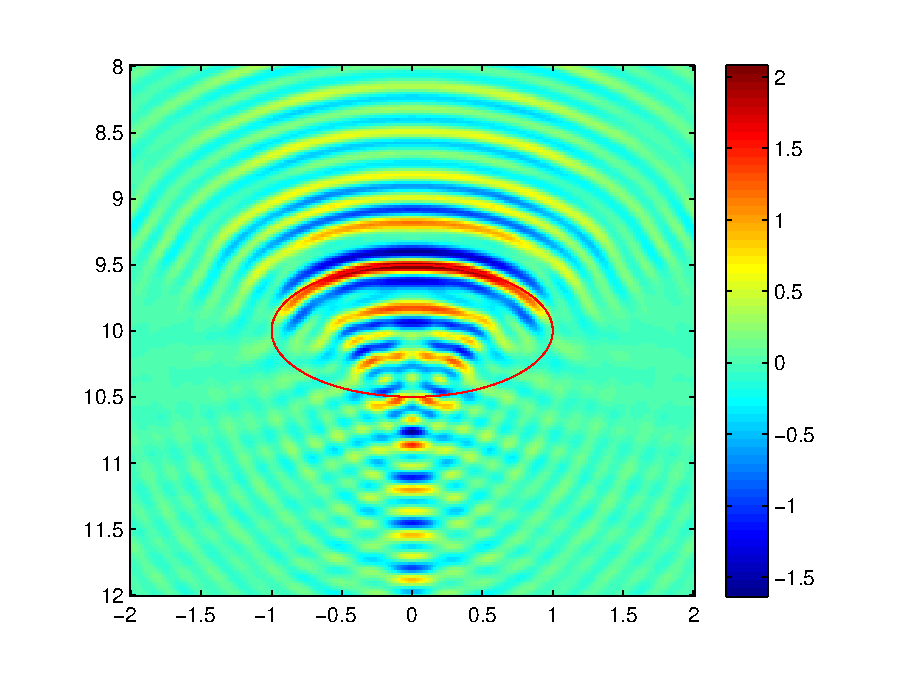
\includegraphics[width=0.32\textwidth]{./graphic/circle_3pi.eps}
	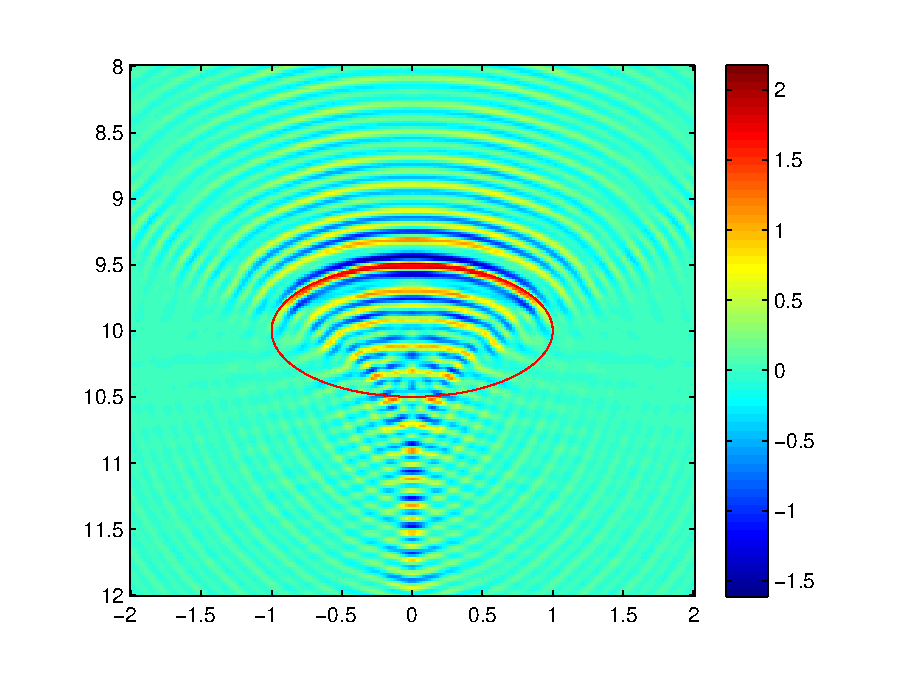
\includegraphics[width=0.32\textwidth]{./graphic/circle_5pi.eps}
	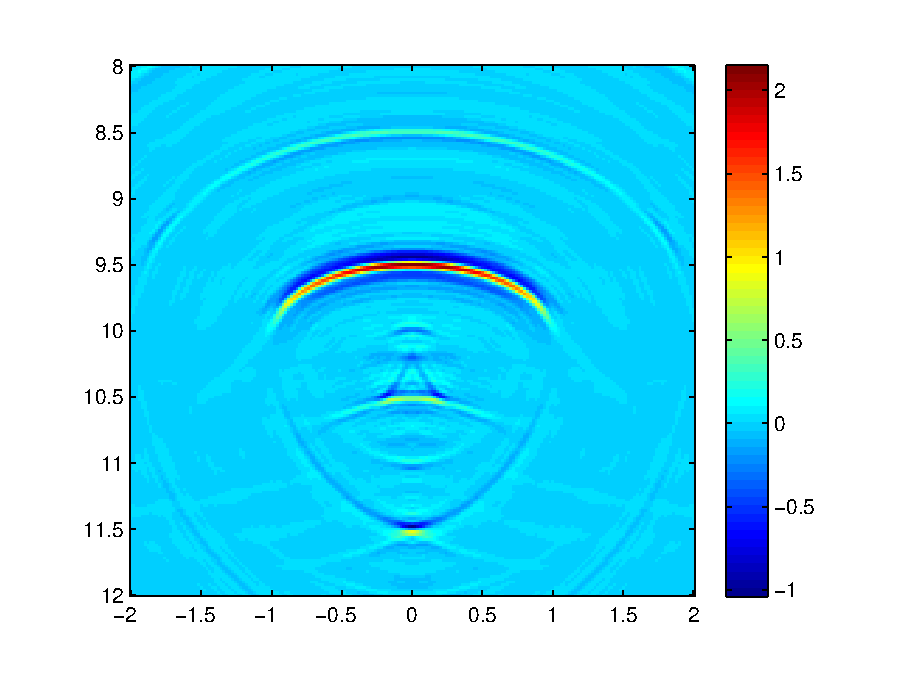
\includegraphics[width=0.32\textwidth]{./graphic/circle.eps}
	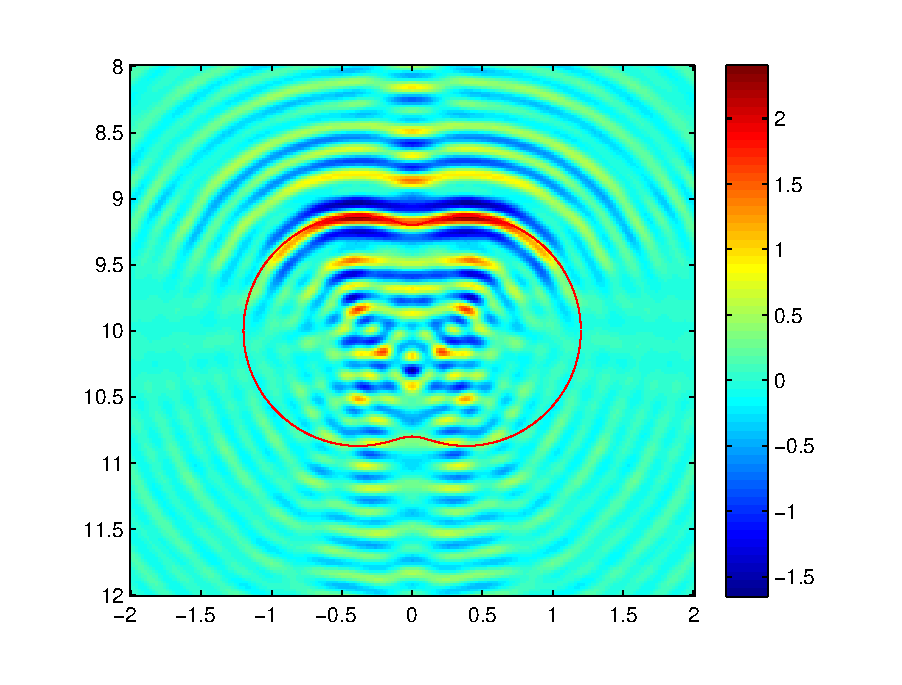
\includegraphics[width=0.32\textwidth]{./graphic/peanut_3pi.eps}
	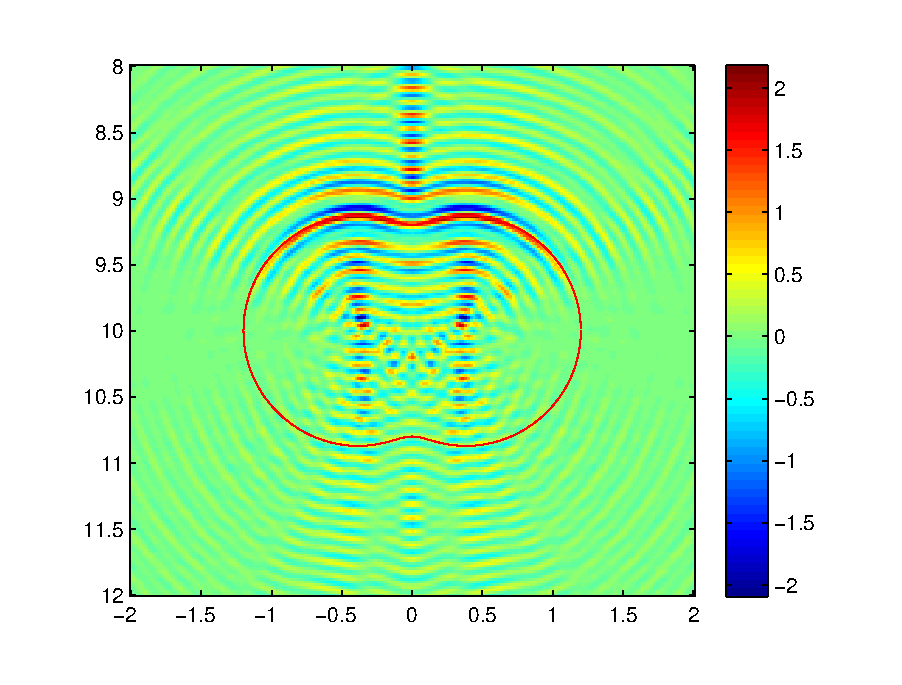
\includegraphics[width=0.32\textwidth]{./graphic/peanut_5pi.eps}
	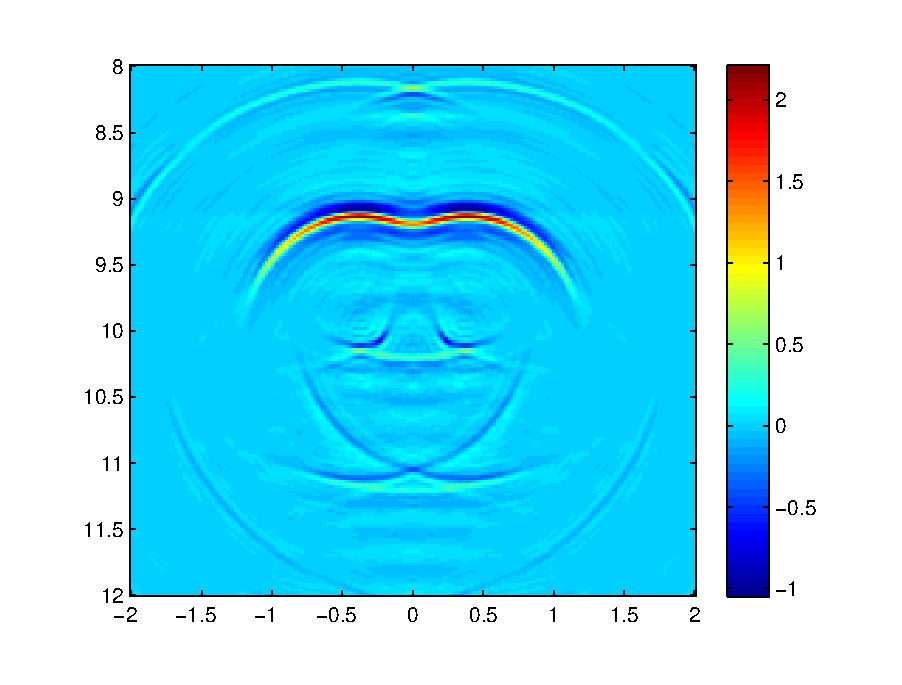
\includegraphics[width=0.32\textwidth]{./graphic/peanut.eps}
	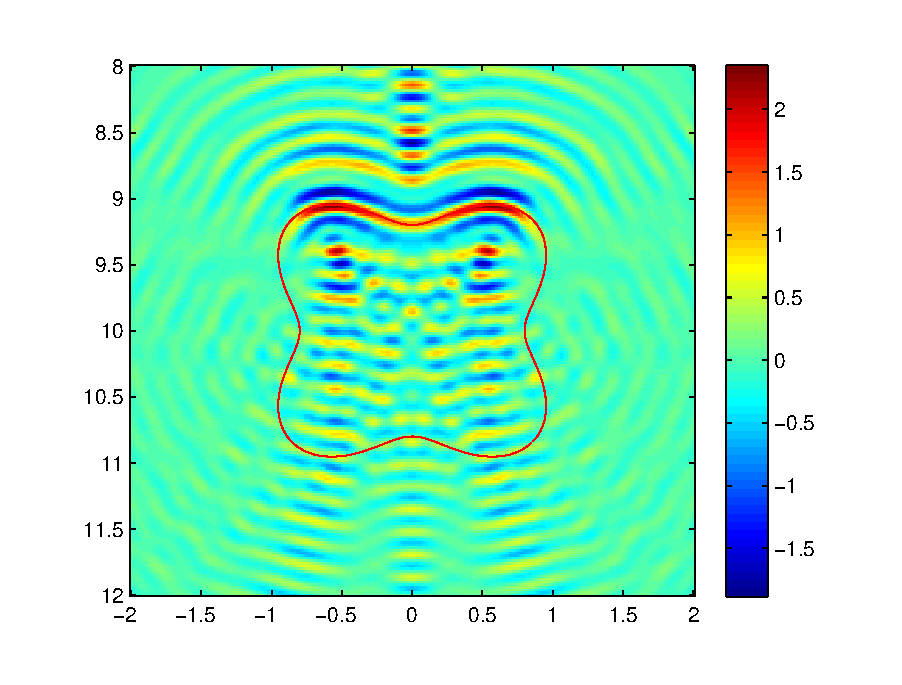
\includegraphics[width=0.32\textwidth]{./graphic/p_leaf_3pi.eps}
	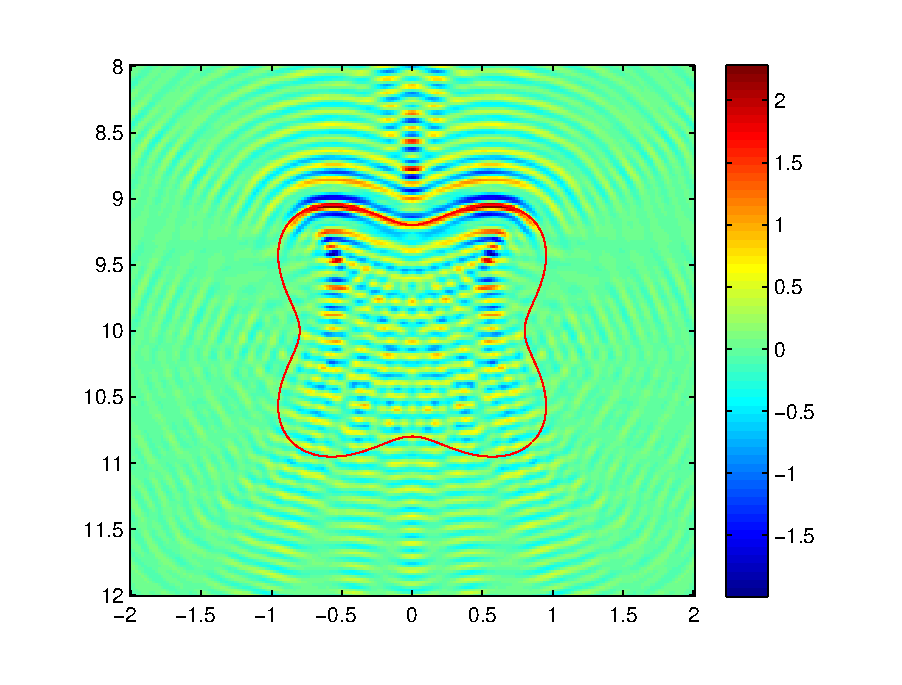
\includegraphics[width=0.32\textwidth]{./graphic/p_leaf_5pi.eps}
	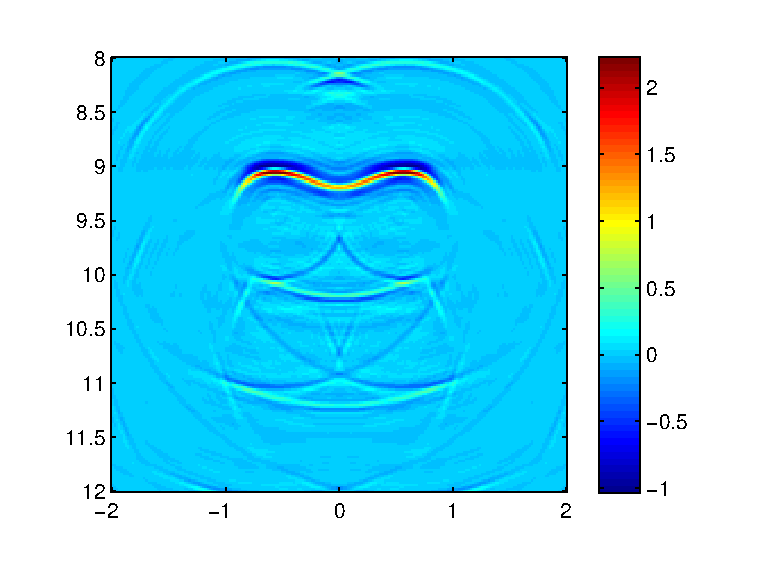
\includegraphics[width=0.32\textwidth]{./graphic/p_leaf.eps}
	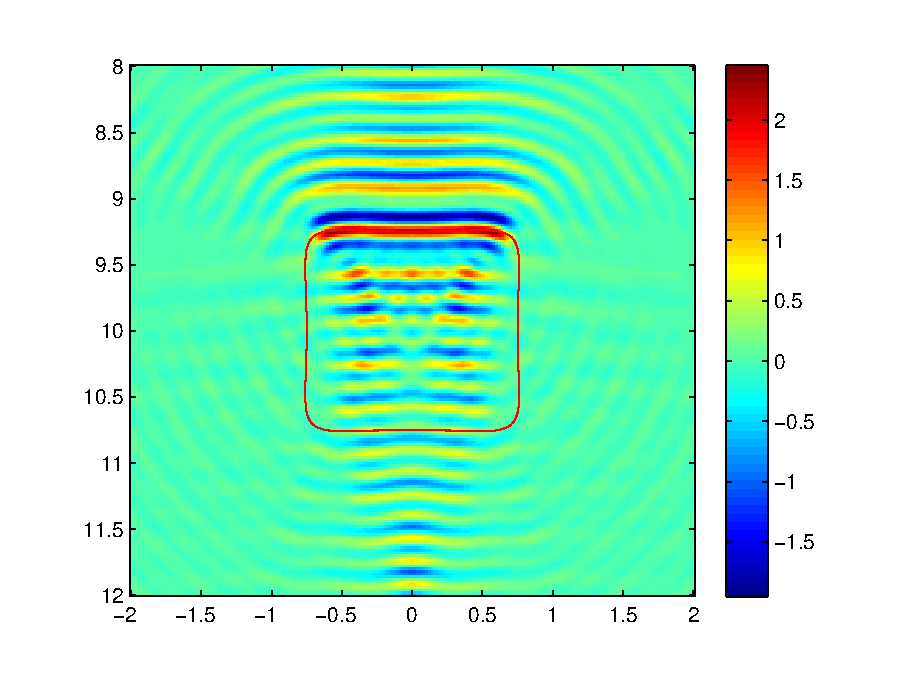
\includegraphics[width=0.32\textwidth]{./graphic/rectangle_3pi.eps}
	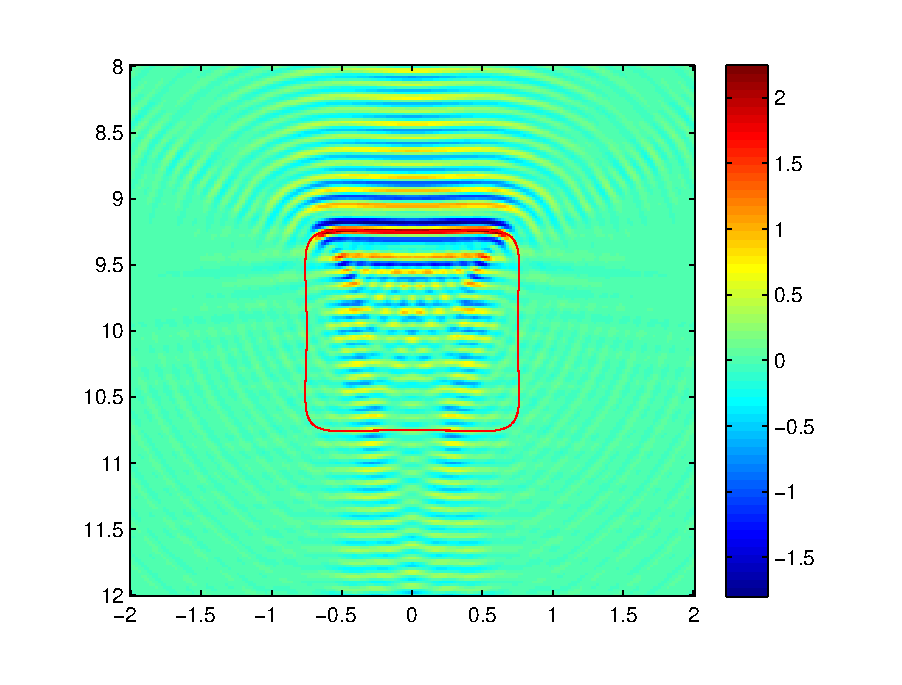
\includegraphics[width=0.32\textwidth]{./graphic/rectangle_5pi.eps}
	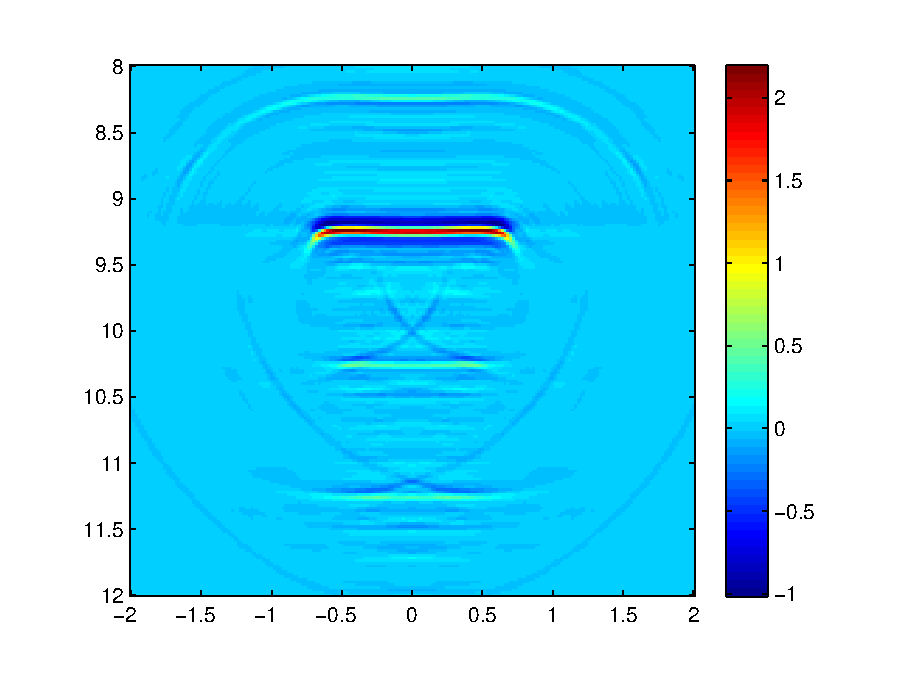
\includegraphics[width=0.32\textwidth]{./graphic/rectangle.eps}
	
	\caption{Example 2: Imaging results of clamped obstacles
		with different shapes from top to below. The left row is imaged with single frequency data where $\om=3\pi$, The middle row is imaged with single frequency data where $\om=5\pi$ and The left row is imaged with multi frequency data}\label{figure_2}
\end{figure}

\bigskip
\textbf{Example 3} We consider the imaging of two sound soft obstacles. The first model
consists of two circles along horizontal direction and the second one is a circle and a
peanut along the vertical direction. The angular frequency is $\om=3\pi$ for the test of the single frequency and $\om=\pi\times[2:0.5:8]$ for the test of multiple frequencies. Figure \ref{figure_31} shows the imaging result of the first model. The
imaging domain is $[−4, 4] \times [8,12]$ with mesh size $401 \times 201$ and $N_s = N_r = 301$. Figure \ref{figure_32}
 shows the imaging result of the second model. The
 imaging domain is $[−4, 4] \times [8,12]$ with mesh size $401 \times 401$ and $N_s = N_r = 301$. The multi-frequency RTM imaging results in Figure \ref{figure_31} and Figure \ref{figure_32} are obtained by adding the inmaging results from different frequencies. We observe from these two figures that imaging results can be greatly improved by stacking the multiple single frequency imaging results. 
\begin{figure}
	\centering
	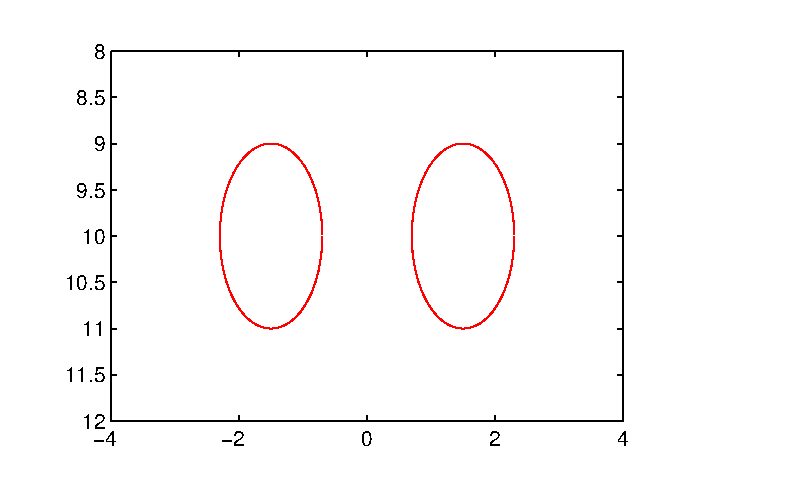
\includegraphics[width=0.32\textwidth,height=0.16\textheight]{./graphic/bi_circle_profile.eps}
	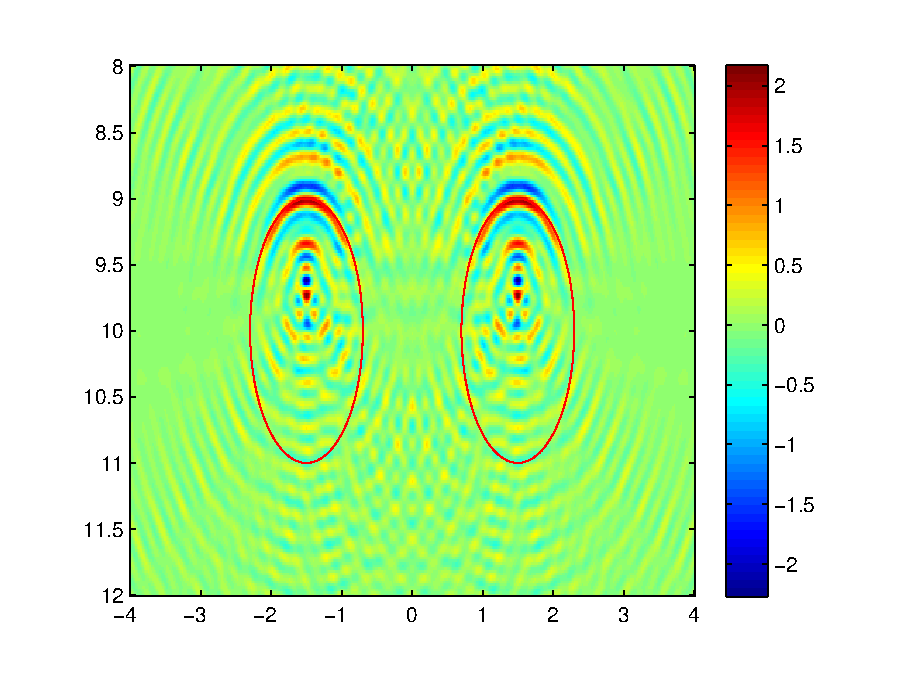
\includegraphics[width=0.32\textwidth]{./graphic/bi_circle_3pi.eps}
	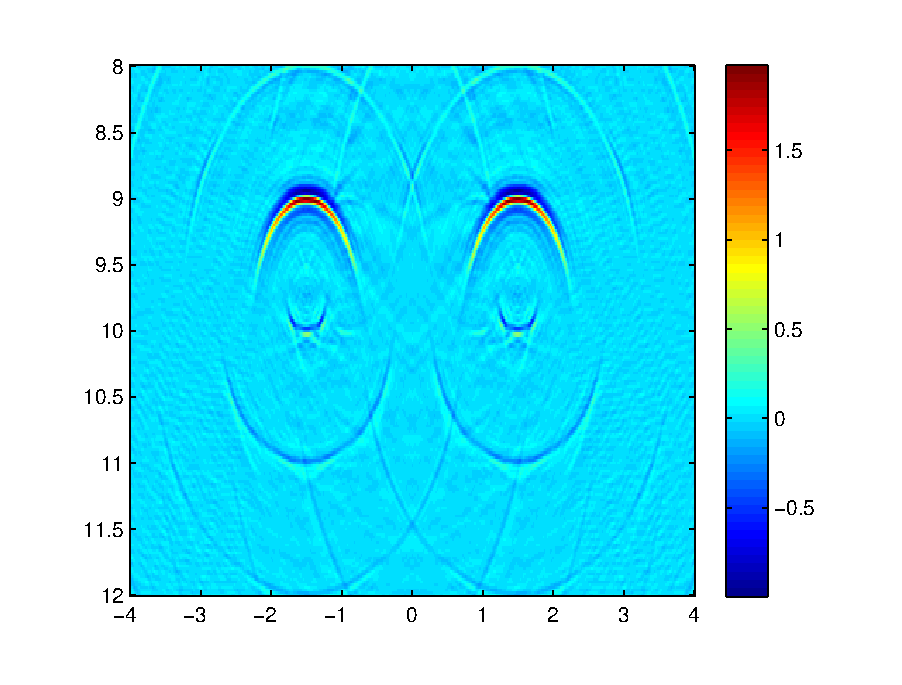
\includegraphics[width=0.32\textwidth]{./graphic/bi_circle.eps}
	
	\caption{Example 3:From left to right,  true obstacle model with two circles. the imaging result
		with single frequency data where $\om=3\pi$, the imaging result with multiple frequency data.}\label{figure_31}
\end{figure}

\begin{figure}
	\centering
	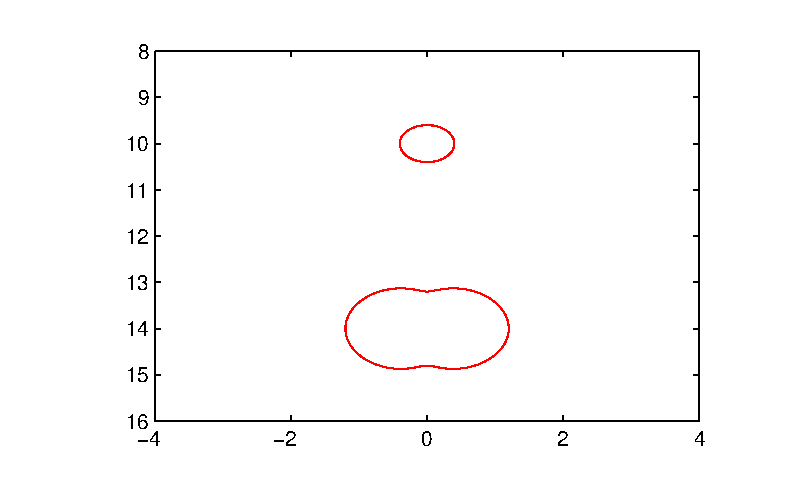
\includegraphics[width=0.32\textwidth,height=0.16\textheight]{./graphic/circle_0_4_peanut_1_profile.eps}
	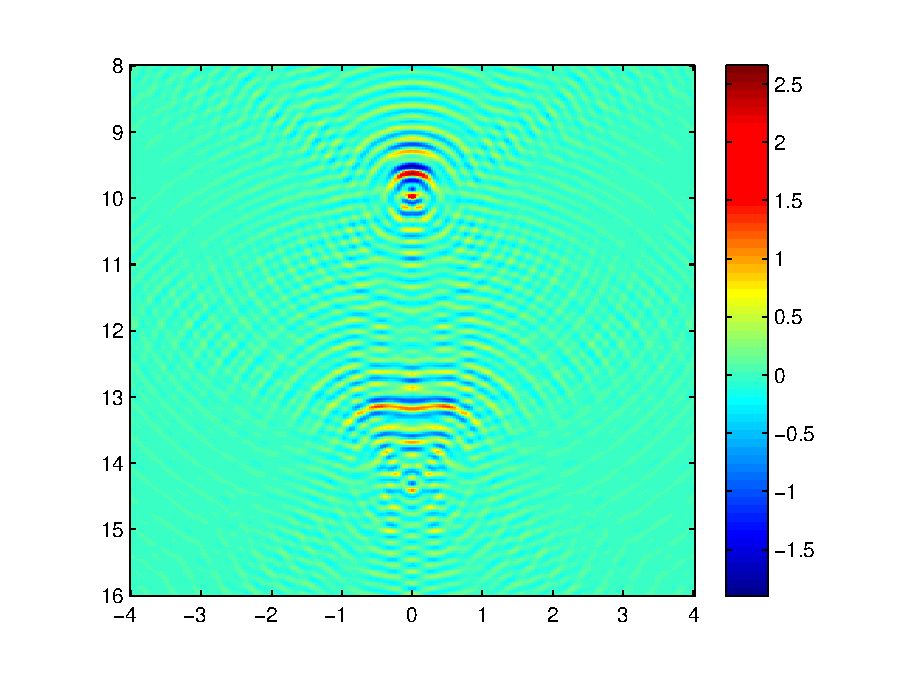
\includegraphics[width=0.32\textwidth]{./graphic/circle_0_4_peanut_1_3pi_1.eps}
	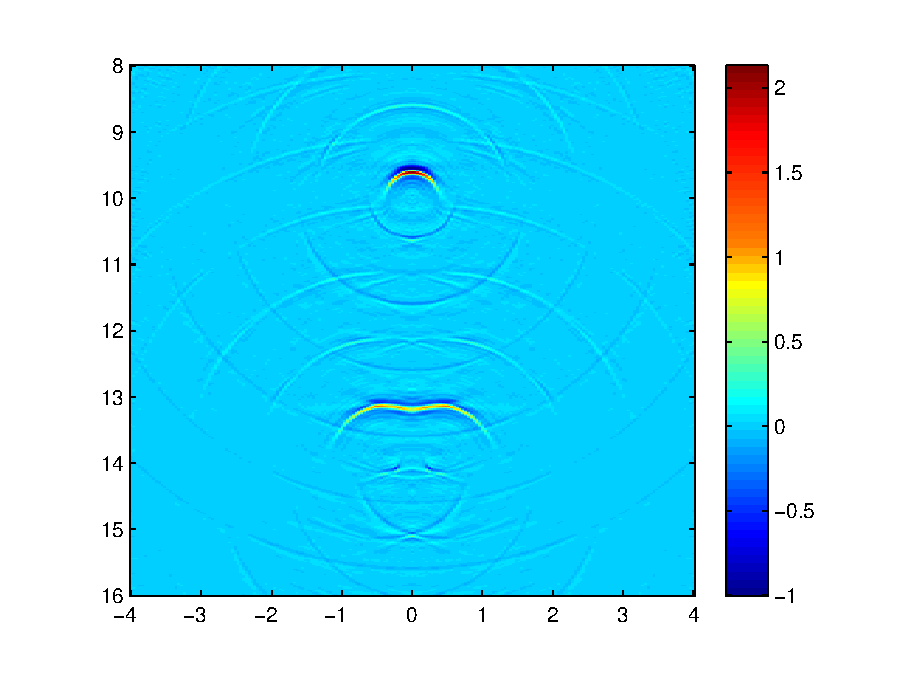
\includegraphics[width=0.32\textwidth]{./graphic/circle_0_4_peanut_1_multi_1.eps}
	
	\caption{Example 3:From left to right,  true obstacle model with one circle and one peanut, the imaging result
		with single frequency data where $\om=3\pi$, the imaging result with multiple frequency data.}\label{figure_32}
\end{figure}

\bigskip
\textbf{Example 4}
In this example we consider the stability of our half space RTM imaging
function with respect to the complex additive Gaussian random noise. We introduce
the additive Gaussian noise as follows
\ben
u_{\rm noise}=u_s+\nu_{\rm noise}
\een
where $u_s$ is the synthesized data and $\nu_{\rm noise}$ is the Gaussian noise with mean zero and standard deviation $\mu$ times the maximum of  the data $|u_s|$, i.e. $\nu_{\rm noise}=\frac{\mu \max |u_s|}{\sqrt{2}}(\ep_1+\i\ep_2)$ and  $\ep_i
\thicksim \mathcal{N}(0,1)$.
\begin{figure}
	\centering
	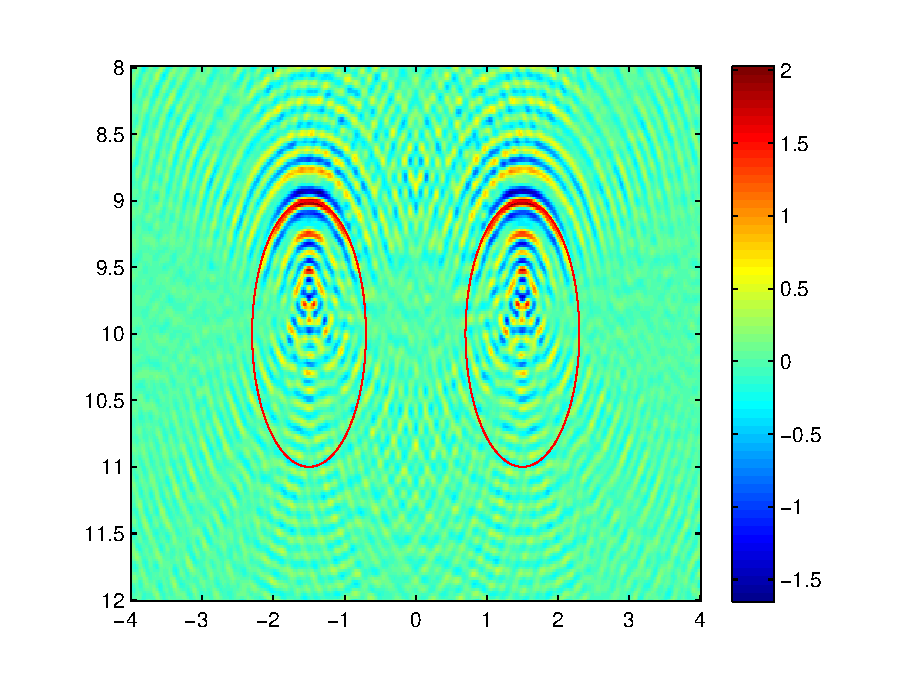
\includegraphics[width=0.32\textwidth]{./graphic/bi_circle_4pi_error2.eps}
	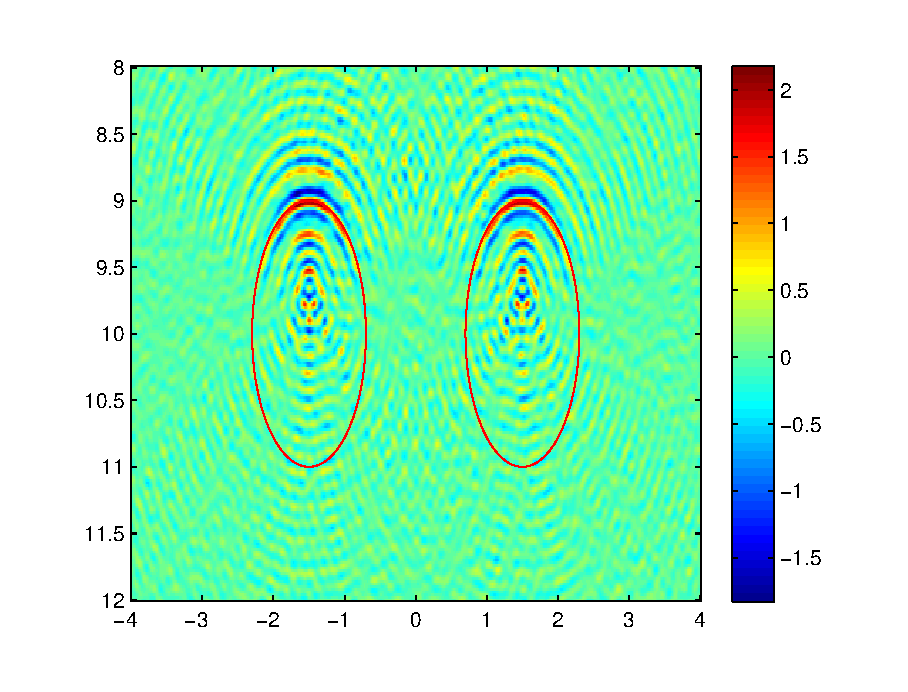
\includegraphics[width=0.32\textwidth]{./graphic/bi_circle_4pi_error4.eps}
	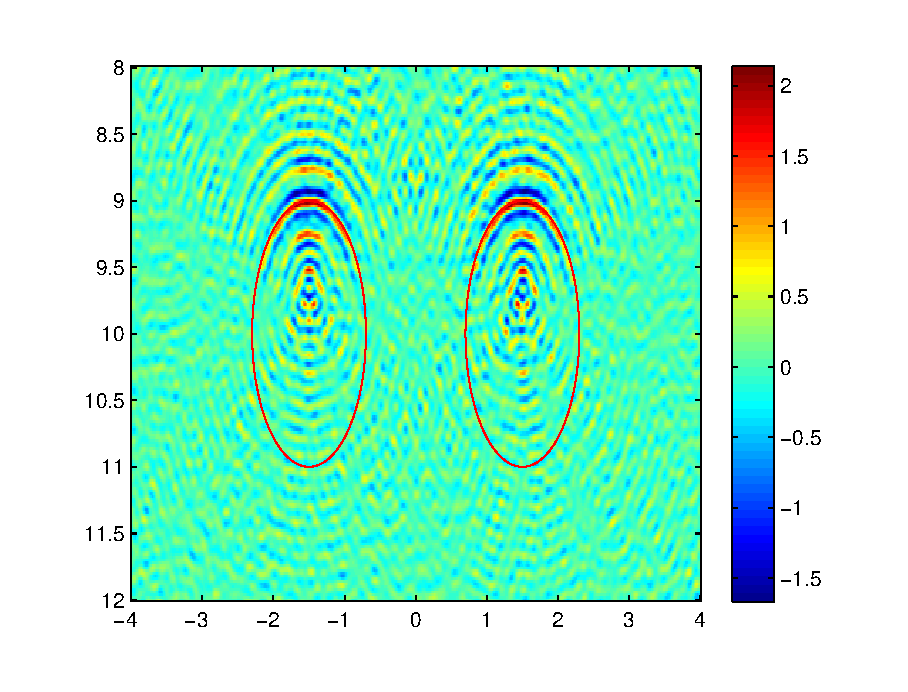
\includegraphics[width=0.32\textwidth]{./graphic/bi_circle_4pi_error6.eps}
	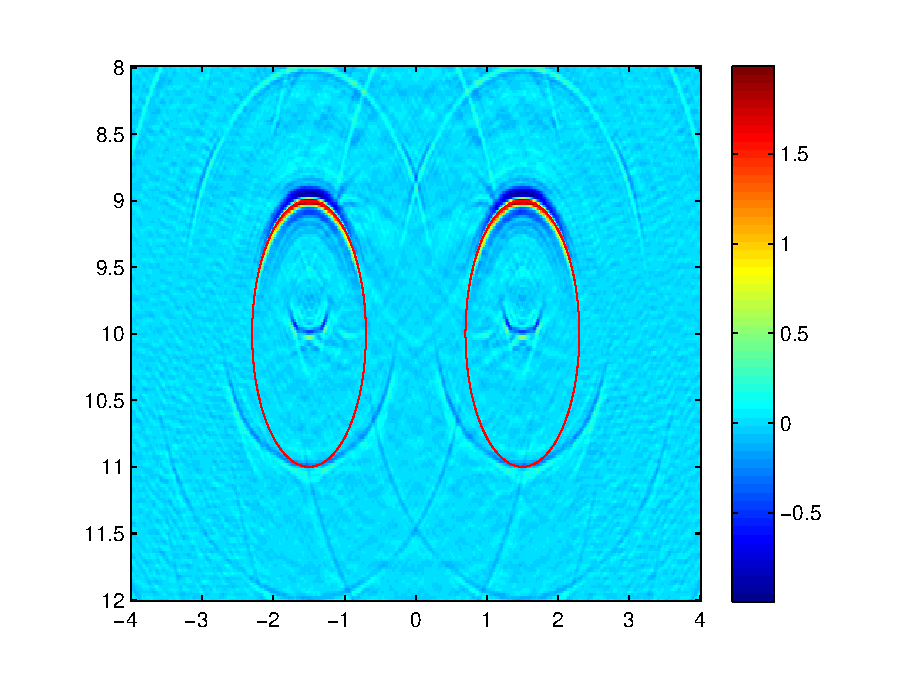
\includegraphics[width=0.32\textwidth]{./graphic/bi_circle_multi_2_8_error2.eps}
	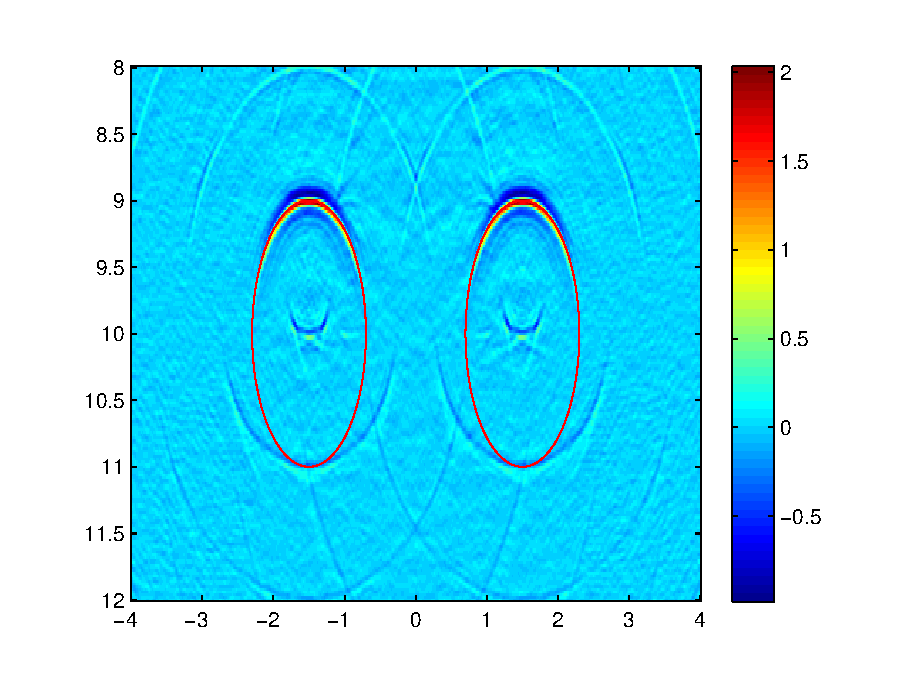
\includegraphics[width=0.32\textwidth]{./graphic/bi_circle_multi_2_8_error4.eps}
	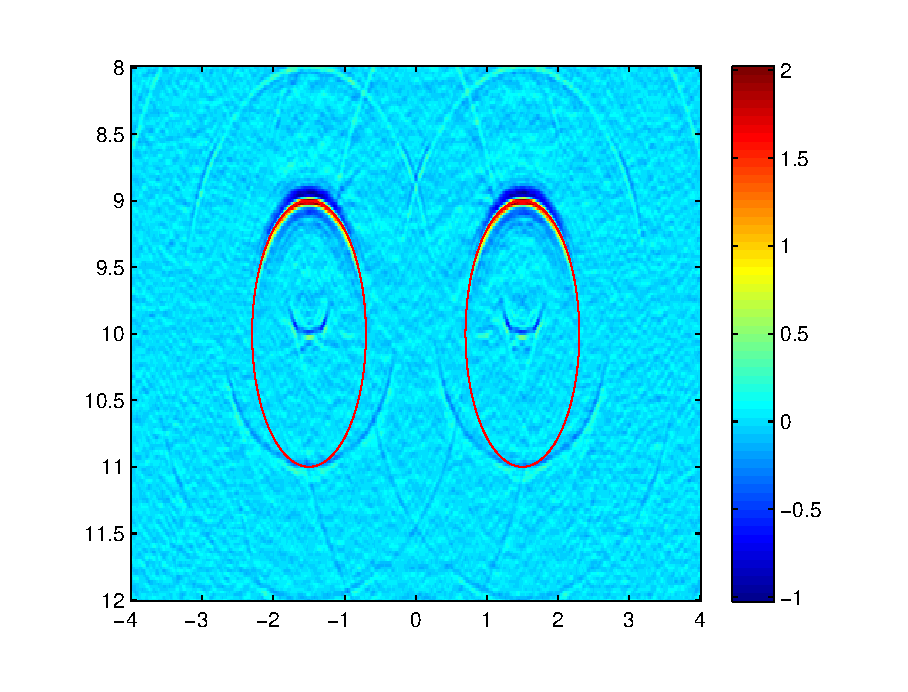
\includegraphics[width=0.32\textwidth]{./graphic/bi_circle_multi_2_8_error6.eps}
	
	\caption{Example 4: Imaging results of a clamped obstacle with noise levels $\mu =  0.2; 0.3; 0.4$ (from left to
		right). The top row is imaged with single frequency data where $\om=4\pi$, and the
		bottom row is imaged with multi-frequency data.}\label{figure_4}
\end{figure}

Figure \ref{figure_4} shows the imaging results using single frequency data added with additive
Gaussian noise. The imaging quality can be improved by using multi-frequency data.
as illustrated 
\section{Appendix A: proof of theorem \ref{elastic_eq2}}

In this section we will prove theorem \ref{elastic_eq2} by extending the classical argument in \cite{leis,wilcox1975,Yves1988}.
The existence of the solution can be proved by the method of limiting absorption principle. The argument is standard and we give several lemmas below, see e.g. \cite{leis} for the consideration for Helmholtz equation. For any $z=1+\i\ep,\ep>0$, $f\in H^{1}(\R^2_+)'$ with compact support in $B_R=\{x||x|^2<R^2,x\in\R^2_+\}\subsetneq\R_+^2$ where $B_R$ is an half disc of radius R , we consider the problem
\be \label{elastic_eqz}
\Delta_e u_z +z\omega^2 u =-f \qquad\mbox{\rm in } \R^2_+ \\
\sigma(u_z)e_2=0 \ \ \ \ \mbox{\rm on} \ \ \ \  \Ga_0 \label{elastic_b0}
\ee
By Lax-Milgrim lemma we know that (\ref{elastic_eqz}-\ref{elastic_b0}) has a unique solution $u_z\in H^1(\R^2_+)$. For any domain $ D \subset \R^2_+$, we define the weighted space $L^{2,s}(D),s \in \R$, by
\ben
L^{2,s}(D)=\{v \in L^2_{\rm loc}(D): (1+|x|^2)^{s/2}v \in L^2(D) \}
\een
with the norm $\| v \|_{ L^{2,s}(\mathcal D)} = (\int_{\mathcal D}(1+|x|^2)^{s}|v|^2 dx )^{1/2}$. The weighted Sobolev space $H^{1,s}(D),s \in \R$,
is defined as the set of functions in $L^{2,s}(D)$ whose first derivative is also in $L^{2,s}(D)$. The norm
$\| v \|_{ H^{1,s}(D)} = (\| v \|^2_{ L^{2,s} (D)} + \| \nabla v \|^2_{ L^{2,s}(D)})^{1/2}$.

We need the following sligt generalization of Rellich Theorem:
\begin{lem}\label{relli_embed}
	Let $\Omega$ be an open Lipschitz domain, then the sobolev space $H^{1,-s}(\Omega)$ is compactly embeded in $L^{2,-s'}(\Omega)$ for every $s'>s>0$.
\end{lem}

\begin{lem}{\label{global_es}}
	Let  $ f  \in L^2 (\R^2_+) $ with compact support in $B_R$. For any $z=1+\i\ep$, $0<\ep<1$, we have, for any $s>1/2$,
	$\|u_z\|_{H^{1,-s}(\R^2_+)}\le C\|f\|_{L^2(\R^2_+)}$ for some constant independent of $\ep, u_z$, and $f$.
\end{lem}
\debproof
Let $R_z$ denote the map from $L^2_c(\R^2_+)$ to $H^{1,-s}(\R^2_+)$ such that $R_z(f)=u_z$ where $L^2_c(\R^2_+)$ is denoted by all $ f  \in L^2 (\R^2_+) $ with compact support in $B_R$, then it is easy to see that $R_z$ is a linear bounded operator. It follows from theorem 3.7 in \cite{Yves1988} that $R_z$ is a uniformly continuous operator continues valued function on $z=1+\i\ep$, $0<\ep<1$ with value in $B(L^2_c(\R^2_+),H^{1,-s}(\R^2_+))$. Then, we can obtain that $R_z$ is uniformly bounded in $B(L^2_c(\R^2_+),H^{1,-s}(\R^2_+))$. This complete the proof by the defintion of the operator norm.
\finproof

We next recall the following lemma which states the absence of positive eigenvalues for the linear elasticity system in half space \cite{sini2004}.
\begin{lem} \label{elas_unique}
	Let $u\in L^2(\R^2_+ \backslash \bar D)$ such that $u$ satisfies (\ref{elas_1}) and (\ref{elas_b0}), than we assert that $u=0$ in $\R^2_+ \backslash \bar D$
\end{lem}
\debproof
The asserting above can be proved by extending \cite[theorem 3.1]{sini2004}, here we omit the details.
\finproof

For any $0<\ep<1$, we consider the problem
\be {\label{elas_z1}}
\Delta_e u_\ep + (1+\i\ep)\omega^2 u_\ep=0 \qquad\mbox{\rm in } \R^2_+\bks \bar{D}\\
u_\ep= g \ \ \ \ \mbox{\rm on } \Ga_D  \label{elas_zbd}\\
\sigma(u_\eps)e_2=0 \ \ \ \ \mbox{\rm on} \Ga_0 \label{elas_zb0}
\ee
We know that the above problem has a unique solution $u_{\ep} \in H^1(\R^2_+ \backslash \bar D)$ by the Lax-Milgram Lemma. Thus, we have next lemma
\begin{lem}{\label{global_elas_bd}}
	Let  $ g  \in H^{1/2} (\Ga_D) $ . For any $0<\ep<1$, we have, for any $s>1/2$,
	$\|u_{\eps}\|_{H^{1,-s}(\R^2_+ \backslash \bar D)} \leq C \|g\|_{H^{1/2}(\Ga_D)}$ for some constant independent of $\ep, u_\eps$, and $g$.
\end{lem}
\debproof
Because $h=dist(D,\Ga_0)>0$, we can find three concentric circles $B_{R_1},B_{R_2},B_{R_3}$ such that $D\subsetneq B_{R_1}\subsetneq B_{R_2} \subsetneq B_{R_3} \subsetneq \R^2_+$. Let $\chi \in C_{0}^{\infty}(\R^2_+)$ be the cut-off function such that $0 \leq \chi \leq 1$, $\chi=0$ in $B_{R_1}$, and $\chi=1$ outside of $B_{R_2}$.
Let $v_\eps=\chi u_\eps$.
Then $v_\eps$ satisfies (\ref{elastic_eqz}) with
$z=1+\i\eps$ and $q=\sigma(u_\eps)\na\chi+(\lambda+\mu)(\na^2 \chi u_\eps+ \na u_\eps \na\chi)+\mu\Delta\chi u_\eps +\mu\div u_\eps\na\chi$, where $\na^2 \chi$ is the Hessian matrix of $\chi$. Clearly $q$ has compact support. By lemma \ref{global_es} we can obtain
\be \label{elas_ineq2}
\|v_\eps\|_{H^{1,-s}(\R^2_+)}\le C\|u_{\eps}\|_{H^1(B_{R_2}\backslash \bar{D})}
\ee
for some constant $C$ independent of $\eps>0$. Now let $\chi_1 \in C_{0}^{\infty}(\R^2_+)$
be the cut-off function with that  $0 \leq \chi_1 \leq 1$, $\chi_1=1$ in $B_{R_2}$, and $\chi_1=0$
outside of $B_{R_3}$. For $g\in H^{1/2}(\Ga_D)$, let $u_g \in H^{1}(\R^2_+ \backslash \bar{D})$ be the lifting function such that $  u_{g}=g \mbox{ on } \Ga_D$ and $\|u_{g}\|_{H^{1}(\R^2_+ \backslash \bar{D})}\le C\|g\|_{H^{1/2}(\Ga_D)}$. By testing \ref{elas_z1} with
$\chi_1^2 ( \overline{u_{\eps}-u_{g}} )$ and using the standard argument we have
\be \label{elas_ineq3}
\|u_{\eps}\|_{H^{1}(B_{R_2} \backslash \bar{D})}\le C( \|u_{\eps}\|_{L^{2}(B_{R_3} \backslash \bar{D})} + \|g\|_{H^{1/2}(\Ga_D)} ).
\ee
A combination of (\ref{elas_ineq2}) and the above estimate yields
\be \label{elas_ineq4}
\|u_{\eps}\|_{H^{1,-s} ( \R^2_+ \backslash \bar{D})}\le C( \|u_{\eps}\|_{L^{2}(B_{R_3} \backslash \bar{D})} + \|g\|_{H^{1/2}(\Ga_D)} ).
\ee
Now we claim
\be \label{elas_ineq5}
\|u_{\eps}\|_{L^2(B_{R_3} \backslash \bar D)} \leq C \|g\|_{H^{1/2}(\Ga_D)} ,
\ee
for any $g \in H^{1/2}(\Ga_D)$ and $\eps >0$. If it were false, there would exist sequences $\{g_m\} \subset H^{1/2}(\Ga_D)$ and $\{\eps_m\} \subset (0,1)$, and $\{u_{\eps_m}\}$ be the corresponding solution of (\ref{elas_z1})-(\ref{elas_zb0}) such that
\be {\label{contradict}}
\|u_{\eps_m}\|_{L^2(B_{R_3} \backslash \bar D)} = 1 \ {\rm{ and }} \ \|g_m\|_{H^{-1/2}(\Ga_D)} \leq \frac{1}{m}.
\ee
Then $\|u_{\eps_m}\|_{H^{1,-s} ( \R^2_+ \backslash \bar{D})}\le C $, and thus there is a subsequence of $\{\eps_m\}$, which is
still denoted by $\{\eps_m\}$, such that $\eps_m \to \eps' \in [0,1]$, and a subsequence of $\{u_{\eps_m}\}$,
which is still denoted by $\{u_{\eps_m}\}$, such that it converges to some $u_{\eps'}$ in ${H^{1,-s'} ( \R^2_+ \backslash \bar{D})}$ by choosing $s'>s$. This is a consequence of Korn's inequality and lemma \ref{relli_embed}. So $u_{\eps'} \in H^{1,-s'}(\R^2_+ \backslash \bar D)$ satisfies (\ref{elas_z1}-\ref{elas_zb0}) with $g=0$ and $\eps=\eps'$.

By the integral representation satistied by $u_{\eps_m}$, we know that for $y\in \R^2_+\backslash\bar B_{R_1}$ and $i=1,2$
\be \ \hspace{-2cm} \label{green_rep}
u_{\eps'}(y)\cdot e^i=\int_{\pa B_{R_1}} (\sigma(N_{\eps'}(x,y)e_i)\nu)\cdot u_{\eps'}(x) - (N_{\eps'}(x,y)e_i)\cdot (\sigma(u_{\eps'})_{\eps'}\nu)ds(x)
\ee
If $\eps'>0$, we deduce  from (\ref{green_rep}) that $u_{\eps'}$ decays exponentially and thus $u_{\eps'} \in H^{1}(\R^2_+\backslash \bar D) $, then $u_{\eps'} =0$ by the uniqueness of the solution in $H^{1}(\R^2_+ \backslash \bar D) $ with positive absorption.
If $\eps'=0$, by the \cite[theorem 5.2]{Yves1988}, we have $u_{\eps'}\in L^2(\R^2_+\bks\bar D)$. Then we conclude $u_{\eps'}=0$ by the lemma \ref{elas_unique}
Therefore, in any case $u_{\epsilon'}=0$, which , however contradicts to \ref{contradict}. This complete the proof.
\finproof
Now we are in the position to prove the exsitence of Theorem \ref{elastic_eq2}.
\begin{lem} \label{elas_exis}
	For any $s>1/2$, $u_\eps:(0,1)\to H^{1,-s}(\R^2_+ \bks \bar D)$ is a uniformly continuous operator valued function. Immediately, $u_{\eps}$ converges to some $u_0$ in $H^{1,-s}(\R^2_+ \bks \bar D)$ and $u_0$ is a solution of (\ref{elas_1}-\ref{elas_ineq}).
\end{lem}
\debproof
We also give a indirect prove here. Let $\delta_0>0$ and $\{\mu_n\}$ and $\{\nu_n\}$ be sequences in $ (0,1) $ such that
\be
|\mu_n-\nu_n|\le 1/n \qquad \mbox{and} \qquad \|u_{\mu_n}-u_{\nu_n}\|_{H^{1,-s}(\R^2_+ \bks \bar D)} \ge \delta_0
\ee
Thus there is a subsequence of $\{\mu_n\}$, which is still denoted by $\{\mu_n\}$, such that $\{\mu_n\}\to \epsilon\in[0,1]$ and also $\{\nu_n\}\to \epsilon$. Then using lemma \ref{global_elas_bd} and the procedure proving it, we get the $u_\epsilon,v_\epsilon \in H^{1,-s'} (\R^2_+ \bks \bar D)$, by choosing $s'>s$, such that
\ben
\|u_{\mu_n}-u_\epsilon\|_{H^{1,-s'}(\R^2_+ \bks \bar D)} \to 0 \\
\|u_{\nu_n}-v_\epsilon\|_{H^{1,-s'}(\R^2_+ \bks \bar D)} \to 0
\een
and $u_\epsilon=v_\epsilon$ by the same arguement in lemma \ref{global_elas_bd} which leads to a contradiction. Thus we have proved $u_\eps$ is uniformly continuously for $\eps \in (0,1)$. Then it is easy to see $u_\eps$ has a limitation in ${H^{1,-s}(\R^2_+ \bks \bar D)} $ and the estimation of $u_0$ can be obtained by (\ref{elas_ineq5}). This completes the proof.
\finproof
It is remain to prove the uniqueness in theorem \ref{elastic_eq2}. Actually, it can be obtained following the existence of solution with any $g\in H^{1/2}(\Ga_D)$.

{\it \bf proof of Theorem \ref{elastic_eq2}}
By the linearity of the problem, it is sufficient to prove that any $u_0$  satisfies the system (\ref{elas_1}-\ref{elas_b0}) with the corresponding homogeneous boundary-value vanishes identically in $\R^2_+\bks \bar D$. For any $y\in \R^2_+\bks \bar D$, there exists $U^s(x,y)$ sataifies (\ref{elas_1}-\ref{elas_b0}) with $g(x)=-N(x,y)$ on $\Ga_D$ following the lemma \ref{elas_exis} and we define $U(x,y)=N(x,y)+U^s(x,y)$. It is easy to see that $U(x,y)$ satifies the generalized radiation condition (\ref{rc}). Thus by the integral representaion of $u_0$, we have
\ben
\lim_{r\to\infty}  \int_{S_r^+} (\sigma(U(x,y)e_i)\nu)\cdot u_0(x) - (U(x,y)e_i)\cdot (\sigma(u_0)\nu)ds(x)=0
\een
Finally, combining $U(x,y)=0,u_0(x)=0$ on $\Ga_D$ and the Green integral theorem we find that
\ben
u_0(y)e_i&=\int_{\R^2_+\bks\bar D} -(\Delta_e (N(x,y)e_i)+\omega^2 N(x,y)e_i)\cdot u_0(x) dx\\
&=\int_{\R^2_+\bks\bar D} \Delta u_0(x)\cdot (N(x,y)e_i)
-\Delta_e (N(x,y)e_i)\cdot u_0(x) \\
&=\int_{\Ga_D} (\sigma(U(x,y)e_i)\nu)\cdot u_0(x) - (U(x,y)e_i)\cdot (\sigma(u_0)\nu)ds(x)=0
\een
Then the desired unique exsitence follows lemma \ref{elas_exis}. This completes the proof of theorem \ref{elastic_eq2}.
\finproof
\section{Appendix B: proof of theorem \ref{diff_solu}}
\begin{lem}\label{es_diri_neu}
	For any $x,y\in D$, let
	\ben
	p(x,y)=\lim_{\ep\to0^+}p^\ep(x,y):=\lim_{\ep\to0^+}\int_\R \frac{f(\mu^\ep_p,\mu^\ep_s,\xi)}{\delta^\ep(\xi)}e^{\i\mu^\ep_\alpha x_2+\i \mu^\ep_\beta y_2+\i \xi(y_1-x_1)}d\xi
	\een
	where $f(a,b,c)$ is a homogeneous fifth order polynomial with repect to a,b,c and $\alpha,\beta\in \{p,s\}$.Then there exists a constant $C>0$ only depandent on $\kappa$ such that
	\ben\hspace{-2.5cm}
	|p(x,y)|+k_s^{-1}|\nabla_x p(x,y)|+k_s^{-1}|\nabla_y p(x,y)|+k_s^{-2}|\nabla_x\nabla_y p(x,y)|\leq C((k_s h)^{-1/2}+k_s he^{-\sqrt{k_R^2-k_s^2}h})
	\een
	uniformly for $x,y\in D$.
\end{lem}
\debproof
Without loss of generality, we assume $k_\alpha\leq k_\beta$. Then we can divide $p(x,y)$ into two parts:
\ben
p(x,y)&=&\lim_{\ep\to0^+}\int_{I_1}+\int_{I_2}\frac{f(\mu^\ep_p,\mu^\ep_s,\xi)}{(k^\ep_\alpha)^2\delta^\ep(\xi)}e^{\i\mu^\ep_\alpha x_2+\i \mu^\ep_\beta y_2+\i \xi(y_1-x_1)}d\xi\\
&=&\int_{I_1}\frac{f(\mu_p,\mu_s,\xi)}{k^2_\alpha\delta(\xi)}e^{\i\mu_\alpha x_2+\i \mu_\beta y_2+\i \xi(y_1-x_1)}d\xi\\
&+&\lim_{\ep\to0^+}\int_{I_2}\frac{f(\mu^\ep_p,\mu^\ep_s,\xi)}{(k^\ep_\alpha)^2\delta^\ep(\xi)}e^{\i\mu^\ep_\alpha x_2+\i \mu^\ep_\beta y_2+\i \xi(y_1-x_1)}d\xi\\
&=&p_1(x,y)+p_2(x,y)
\een
where $I_1=(-k_\alpha,k_\alpha)$ and $I_2=R\bks[-k_\alpha,k_\alpha]$. Substituting $\xi=k_\alpha t$ into $p_1(x,y)$, we get
\ben
p_1(x,y)=\int_{-1}^{1}\frac{ f(\mu_p(k_\alpha t),\mu_s(k_\alpha t),k_\alpha t)}{k_\alpha \delta(k_\alpha t)}e^{\i k_\alpha x_2(\sqrt{1-t^2}+\tau \sqrt{\varsigma^2-t^2} +\gamma t)}dt
\een
where $\tau=y_2/x_2$, $\varsigma=k_\beta/k_\alpha$ and $\gamma=(y_1-x_1)/x_2$. It is easy to see that the phase function $\phi(t)=\sqrt{1-t^2}+\tau \sqrt{\varsigma^2-t^2} +\gamma t$ satifies $|\phi''(t)|\geq 1/(1-t^2)^{3/2}\geq1$ for $t\in(-1,1)$. Then we can obtain $|p_1(x,y)|\leq C 1/(k_s h)^{1/2}$ by lemma \ref{van}.

For $p_2(x,y)$, by the defination of Cauchy priciple value and lemma \ref{pv_term} and lemma \ref{medi_term}, we can easily obtain:
\ben
|p_2(x,y)|\leq C(\frac{1}{k_sh}+k_s he^{-\sqrt{k_R^2-k_s^2}}h)
\een
This completes the proof of the esitmate for $|p(x,y)|$. The other estimates can be proved by a similar argument. We omit the details here.
\finproof

Now we are ready to prove Theorem \ref{diff_solu}.\\
{\it \bf proof of Theorem \ref{diff_solu}}
Denote by $u_1^\ep$, $u_2^\ep$ the corresponding solution of equations \ref{elas_r1},\ref{elas_r2} where $\om$ is substituted by $\om(1+\i\ep)$ for any $0<\ep<1$. Let $w^\ep(x)$ be the solution of the problem:
\be {\label{elas_z3}}
\Delta_e w^\ep + (1+\i\ep)\omega^2 w^\ep=0 \qquad\mbox{\rm in } \R^2_+\\
\sigma(w^\ep)e_2=-\sigma(u_2^\ep)e_2 \ \ \ \ \mbox{\rm on} \Ga_0 \label{elas_zb01}
\ee
Then $u^\ep_1-u^\ep_2-w^\ep$ satisfies (\ref{elas_z1}),(\ref{elas_zb0}) with the boundary condition $u^\ep_1-u^\ep_2-w^\ep=-w^\ep$ on $\Gamma_D$. Thus by the limiting absorption principle, lemma \ref{elas_bd} and trace therorem, we have
\be\label{diff1}
\|\sigma_x(u^\ep_1-u^\ep_2)\nu\|_{H^{-1/2}(\Gamma_D)}&\leq& C(\| w^\ep\|_{H^{1/2}(\Gamma_D)}+|T_x^\nu(w^\ep)\|_{H^{-1/2}(\Gamma_D)})\\
&\leq&C (1+\|T_h^\ep\|)\max_{x\in D}(|w^\ep(x)|+d_D|\nabla w^\ep(x|)
\ee
where C is indepandent of $\ep,\om$. By the integral representation formula we have for any $z\in\Ga_0$
\be
u_2^\ep(z)\cdot e_i=\GG(u_2^\ep(\cdot),\Phi(\cdot,z)e_i)\\
\sigma^\ep(z)\cdot e_i==\GG(u_2^\ep(\cdot),[\sigma_z(\Phi^T(\cdot,z)e_1)e_2\cdot e_i),\sigma_z(\Phi^T(\cdot,z)e_2)e_2\cdot e_i]^T)
\ee
which yields by using the integral representation again that for $x\in D$
\be
w^\ep(x)\cdot e_j=\int_{\Ga_0} N^\ep(z,x) e_j\cdot(\sigma_z(u_2^\ep(z))e_2)ds(z)\\
=\GG(u_2^\ep(\cdot),v^\ep(x,\cdot)e_j)
\ee
where
\be
e_i^Tv^\ep(x,y)e_j=\int_{\Ga_0} N^\ep(z,x)e_j\cdot(\sigma_z(\Phi^\ep(z,y)e_i)e_2)ds(z)
\ee
Since $\|\sigma(u^\ep_2)\nu\|_{H^{-1/2}(\Gamma_D)}\leq \|T_f^\ep\| \|g\|_{H^{1/2}(\Gamma_D)}$, we obtain
\be
|w^\ep(x)|\leq C (1+\|T_f^\ep\|) \|g\|_{H^{1/2}(\Gamma_D)}\max_{x\in D}(|v^\ep(x,y)|+d_D|\nabla_yv^\ep(x,y)|)
\ee
and
\be\hspace{-2cm}
|\nabla w^\ep(x)|\leq C (1+\|T_f^\ep\|) \|g\|_{H^{1/2}(\Gamma_D)}\max_{x\in D}(|\nabla_x v^\ep(x,y)|+d_D|\nabla_x\nabla_yv^\ep(x,y)|)
\ee\hspace{-1.5cm}
By (\ref{diff1}) and letting $\ep\to0^+$, we have 
\be\label{diff2}
\|\sigma(u_1-u_2)\nu\|_{H^{-1/2}(\Gamma_D)}
\leq C(1+\|T_f\|)(1+\|T_h\|)\|g\|_{H^{1/2}(\Gamma_D)}\\
\hspace{-1.5cm}\max_{x\in D}\lim_{\ep\to0^+}(|v^\ep(x,y)|
+d_D|\nabla_y v^\ep(x,y)|+d_D|\nabla_x v^\ep(x,y)|+d_D^2|\nabla_x\nabla_yv^\ep(x,y)|)
\ee
Applying the Fourier transformation to the first horizontal variable of $T_z^{e_2}\Phi^\ep(z,y)$, we have 
\ben \hspace{-2cm}
\mathcal{F}[T_z^{e_2}\Phi^\ep](\xi,0;y)=\frac{\mu}{2\omega^2}
\Bigg[
\Bigg( \begin{array}{cc}
	2\xi^2 & -2\xi\mu_p\\
	-\frac{\beta\xi}{\mu_p} & \beta
\end{array} \Bigg) e^{\i\mu_py_2}+
\Bigg( \begin{array}{cc}
	\beta & \frac{\xi\beta}{\mu_s} \\
	2\xi\mu_s & 2\xi^2
\end{array} \Bigg)e^{\i\mu_s y_2}  \Bigg]e^{-\i\xi y_1}
\een
Using Parseval identity combined with above formula and formula \ref{ngreen}, we have
\ben
\lim_{\ep\to0^+}v^\ep(x,y)=\lim_{\ep\to0^+}\int_{\R}\mathcal{F}[N^\ep](\xi,0;x)^T\mathcal{F}[T_z^{e_2}\Phi^\ep](-\xi,0;y)d\xi
\een
This completes the proof by using lemma \ref{es_diri_neu}.
\finproof
\section*{References}
\begin{thebibliography}{99}
	\bibitem{achenbach1980}
	J. Achenbach 1980 {\em Wave Propagation in Elastic Solids }(North-Holland)
	
	\bibitem{Ahlfors1979Complex}
	L V. Ahlfors 1979 {\em Complex Analysis: An introduction to the theory of analytic functions of one complex variable }(McGraw-Hill)
	
	\bibitem{ammari2013mathematical}
	H. Ammari, J. Garnier, W. Jing, H. Kang, M. Lim, K. Solna, and H. Wang 2013 {\em Mathematical and Statistical Methods for Multistatic Imaging} (Springer)
	
	\bibitem{arens1999}
	T. Arens 1999 {A New Integral Equation Formulation for the Scattering of Plane Elastic Waves by Diffraction Gratings} {\bf 11} 232-245.
	
	\bibitem{baysal1983reverse}
	Baysal E, Kosloff D D, Sherwood J W C. 1983 {Reverse time migration} {\bf 48} 1514--1524.
	
	\bibitem{bleistein2013mathematics}
	Bleistein N, Cohen J and Stockwell J 2001 {\em Mathematics of Multidimensional Seismic Imaging, Migration, and Inversion} (New York: Springer)
	
	\bibitem{berkhout2012seismic}
	{Berkhout A}  1984 {\em Seismic Migration: Imaging of Acoustic Energy by Wave Field Extrapolation}  (New York: Elsevier)
	
	\bibitem{chang1987elastic}
	Chang W, McMechan G A. 1987 {Elastic reverse-time migration} {\it Geophysics} {\bf 48}  1365-1375
	
	\bibitem{chen2013reverse_acou}
	Chen J,  Chen Z and  Huang G 2013 {Reverse time migration for extended obstacles: acoustic waves}  {\it Inverse Problems} {\bf 29}  085005 (17pp)
	
	\bibitem{chen2013reverse_elec}
	Chen J,  Chen Z and  Huang G 2013 {Reverse time migration for extended obstacles: electromagnetic waves} {\it Inverse Problems}
	{\bf 29} 085006 (17pp)
	
	\bibitem{chen2015reverse_elas}
	Chen Z  and  Huang G 2014 {Reverse time migration for extended obstacles: Elastic waves} (in Chinese){\it Science China Mathematics} {\bf 45} 1103--1114
	
	\bibitem{chen2015reverse_planar}
	Chen Z  and  Huang G 2014 {Reverse time migration for reconstructing extended obstacles in planar acoustic waveguides} {\it Science China Mathematics} {\bf 58} 1811-1834
	
	\bibitem{RTMhalf_aco}
	Chen Z and  Huang G 2015 {Reverse time migration for reconstructing extended obstacles in the half space}  {\it Inverse Problems} {\bf 31 }  055007 
	
	\bibitem{chung2012implementation}
	Chung W, Pyun S, Bae H S, et al. 2012{Implementation of elastic reverse-time migration using wavefield separation in the frequency domain} {\it Geophysical Journal International} {\bf 189} 1611--1625
	
	\bibitem{claerbout1985imaging}
	{ Claerbout J F } 1985  { \em Imaging the Earth's Interior} (Oxford: Blackwell Scientific Publication)
	
	\bibitem{colton-kress}
	Colton D  and   Kress R 1998 {\em Inverse Acoustic and Electromagnetic Scattering Problems } (Heidelberg: Springer)
	
	\bibitem{denli2008elastic}
	H. Denli, L. Huang 2008
	{Elastic-wave reverse-time migration with a wavefield-separation imaging condition}
	{\it 78th Annual International Meeting, SEG, Expanded Abstracts} 2346-2350
	
	\bibitem{Yves1988}
	Y. Dermenjian, J. C. Cuillot 1998
	{Scattering of elastic waves in a perturbed isotropic half space with a free boundary. The limiting absorption principle}
	{\it Mathematical Methods in the Applied Sciences} {\bf 10} 87-124
	
	\bibitem{nedelec2011}
	Duran M, Muga I, Nedelec J C. 2011
	{The outgoing time-harmonic elastic wave in a half-plane with free boundary}
	{\it SIAM Journal on Applied Mathematics} {\bf 71} 255-277
	
	\bibitem{grafakos}
	{Grafakos L} 2004 {\em Classical and Modern Fourier Analysis } (London: Pearson)
	
	\bibitem{Harris2001Linear}
	J. Harris 2001 {\em Linear elastic waves} {(Cambridge University Press)}
	
	\bibitem{kupradze1963progress}
	Kupradze V D, Dneddon T Nm Hill R. 1963 {\em Progress in solid mechanics: Dynamical problems in elasticity} {(North-Holland Publishing Company)}
	
	\bibitem{leis}
	{Leis R} 1986 {\em Initial Boundary Value Problems in Mathematical Physics} {(Stuttgart: B.G. Teubner)}
	
	\bibitem{Guzina2006}
	Madyarov A I, Guzina B B. 2006 {A Radiation Condition for Layered Elastic Media} {\it Journal of Elasticity} {\bf 82} 73-98
	
	\bibitem{sini2004}
	M Sini  2004 {Absence of positive eigenvalues for the linearized elasticity system} {\bf 49} 255--277
	
	\bibitem{wilcox1975}
	{ Wilcox C H.} 2006 {\em Scattering theory for the d'Alembert equation in exterior domains}  {(Springer)}
	
	\bibitem{Zhang08}
	Zhang Y and Sun J 2009 {Practicle issues in reverse time migration: true amplitude gathers, noise removal and harmonic source encoding}
	{\it First Break} {\bf 26}  29-35
	
	\bibitem{Zhang2007}
	Zhang Y, Xu S, Bleistein N and Zhang G 2007 {True-amplitude, angle-domain, common-image gathers from one-way wave-equation migration}
	{\it Geophysics} {\bf 72} S49-S58
	
\end{thebibliography}
\end{document}
